\newpage


Oxford M5 - Multivariable Calculus\footnote{\url{https://courses.maths.ox.ac.uk/node/5652}}


\section{Sheet 1}

\subsection{}
\begin{mdframed}
  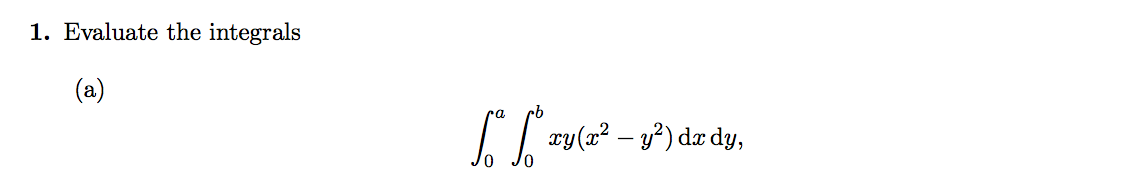
\includegraphics[width=400pt]{img/oxford-prelims-M5-multivariable-calc-1-1-a.png}
\end{mdframed}

\begin{align*}
  \int_0^a\int_0^b xy(x^2 - y^2)\dx\dy
  &= \int_0^a\int_0^b x^3y - xy^3\dx\dy\\
  &= \int_0^a\frac{b^4}{4}y - \frac{b^2}{2}y^3\dy\\
  &= \frac{a^2b^4}{8} - \frac{a^4b^2}{8} \checkmark
\end{align*}

\begin{verbatim}
#+begin_src mathematica
Integrate[x y (x^2 - y^2), {x, 0, b}, {y, 0, a}]
#+end_src

#+RESULTS:
: (-(a^4*b^2) + a^2*b^4)/8

\end{verbatim}


\newpage
\begin{mdframed}
  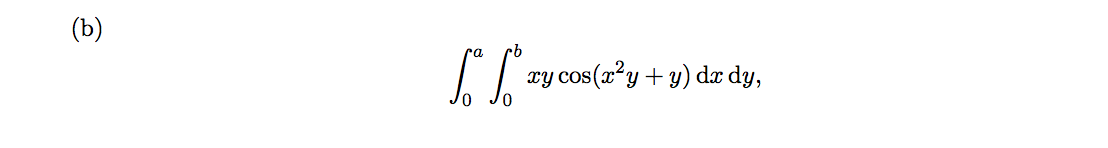
\includegraphics[width=400pt]{img/oxford-prelims-M5-multivariable-calc-1-1-b.png}
\end{mdframed}

Let $u = x^2$ so that $\dxdu = \frac{1}{2x}$. Then

\begin{align*}
  \int_0^a\int_0^b xy\cos(x^2y + y)\dx\dy
  &= \int_0^a\int_0^b xy\cos(uy + y)\dxdu \du\dy\\
  &= \frac{1}{2}\int_0^a\int_{x=0}^{x=b} y\cos(uy + y) \du\dy\\
  &= \frac{1}{2}\int_0^a\Big[\sin(uy + y) \Big]_{u=0}^{u=b^2}\dy\\
  &= \frac{1}{2}\int_0^a\Big[\sin(y(b^2 + 1)) - \sin(y)\Big]\dy\\
  &= \frac{1}{2}\Big[\frac{-\cos(y(b^2 + 1))}{b^2 + 1} + \cos(y)\Big]_{y=0}^{y=a}\\
  &= \frac{1}{2}\Big[\frac{-\cos(a(b^2 + 1))}{b^2 + 1} + \cos(a) +
                     \frac{1}{b^2 + 1} - 1 \Big]\\
  &= \frac{1}{2}\Big[\frac{1 -\cos(a(b^2 + 1))}{b^2 + 1} + \cos(a) - 1 \Big]\\
  &= \frac{1}{2}\Big[\cos(a) - \frac{b^2 + \cos(a(b^2 + 1))}{b^2 + 1} \Big]. \checkmark
\end{align*}

\newpage
\subsection{}
\begin{mdframed}
  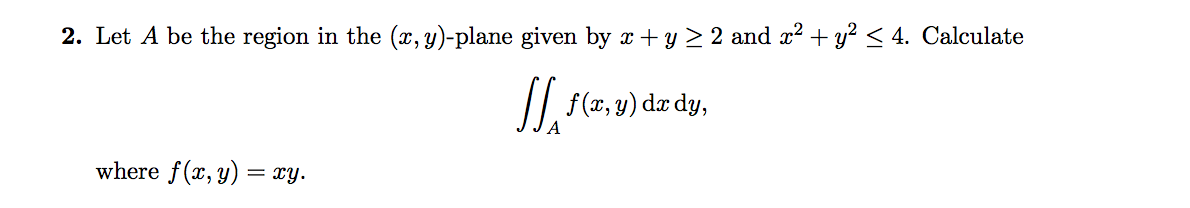
\includegraphics[width=400pt]{img/oxford-prelims-M5-multivariable-calc-1-2.png}
\end{mdframed}
\begin{align*}
     \int_0^2 \int_{2 - x}^{\sqrt{4 - x^2}} xy \dy \dx
  &= \frac{1}{2}\int_0^2 \Big[xy^2\Big]_{y=2 - x}^{y=\sqrt{4 - x^2}} \dx\\
  &= \frac{1}{2}\int_0^2 \Big[x(4 - x^2) - x(2 - x)^2\Big] \dx\\
  &= \frac{1}{2}\int_0^2 x(2-x)\Big[(2 + x) - (2 - x)\Big] \dx\\
  &= \frac{1}{2}\int_0^2 2x^2(2-x) \dx\\
  &= \int_0^2 2x^2 - x^3 \dx\\
  &= \Big[\frac{2}{3}x^3 - \frac{1}{4}x^4\Big]_0^2 \dx\\
  &= \frac{16}{3} - \frac{16}{4}\\
  &= \frac{64 - 48}{12}\\
  &= \frac{4}{3} \checkmark
\end{align*}


\newpage
\subsection{}
\begin{mdframed}
  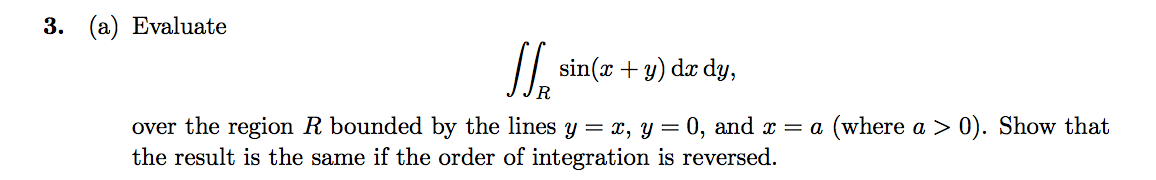
\includegraphics[width=400pt]{img/oxford-prelims-M5-multivariable-calc-1-3-a.png}
\end{mdframed}

\begin{enumerate}[label=(\alph*)]
\item
  \begin{align*}
    \int_0^a \int_y^a \sin(x + y) \dx \dy
    &= -\int_0^a \Big[\cos(x + y)\Big]_{x=y}^{x=a} \dy\\
    &= -\int_0^a \cos(a + y) - \cos(2y) \dy\\
    &= \Big[-\sin(a + y) + \sin(2y)\frac{1}{2}\Big]_0^a \\
    &= -\sin(2a) + \sin(2a)\frac{1}{2} + \sin(a)\\
    &= -\frac{1}{2}\sin(2a) + \sin(a)\\
    &= -\sin(x)\cos(a) + \sin(a)\\
    &= \sin(a)(1 - \cos(a)) \checkmark
  \end{align*}

\begin{verbatim}
#+begin_src mathematica
Integrate[Sin[x + y] Boole[x > y],
          {x, 0, a}, {y, 0, Infinity}, Assumptions -> {a > 0}]
#+end_src

#+RESULTS:
: -((-1 + Cos[a])*Sin[a])

\end{verbatim}

  \newpage
\item~\\
  \begin{mdframed}
    
\includegraphics[width=400pt]{img/oxford-prelims-M5-multivariable-calc-1-3-b.png}
  \end{mdframed}
  \begin{align*}
    \int_0^a\int_0^x f(y) \dy \dx
    &= \int_0^a f(y) \int_y^a \dx \dy\\
    &= \int_0^a f(y) (a - y) \dy\\
  \end{align*}
\end{enumerate}

\newpage
\subsection{}

\begin{mdframed}
  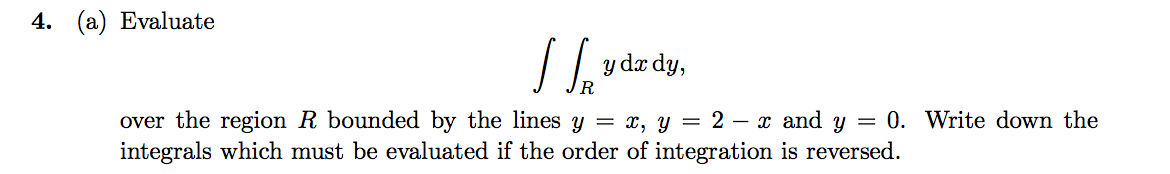
\includegraphics[width=400pt]{img/oxford-prelims-M5-multivariable-calc-1-4-a.png}
\end{mdframed}

\begin{align*}
  I &= \int\int_R y \dx \dy \\
    &= \int_0^1 y \int_y^{2-y} 1 \dx \dy \\
    &= \int_0^1 y [x]_y^{2-y} \dy \\
    &= 2\int_0^1 y \dy \\
    &= 1.
\end{align*}

\begin{mdframed}
  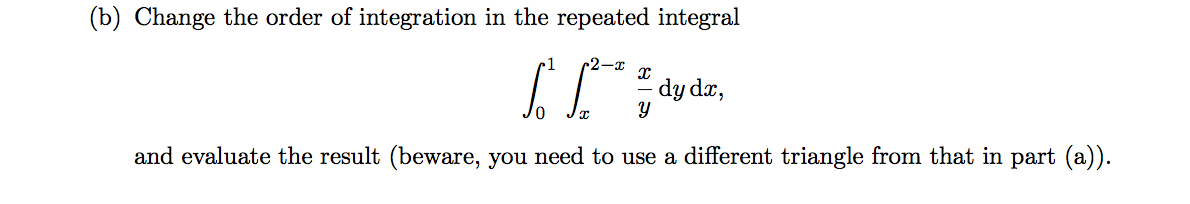
\includegraphics[width=400pt]{img/oxford-prelims-M5-multivariable-calc-1-4-b.png}
\end{mdframed}

\subsection{}
\begin{mdframed}
  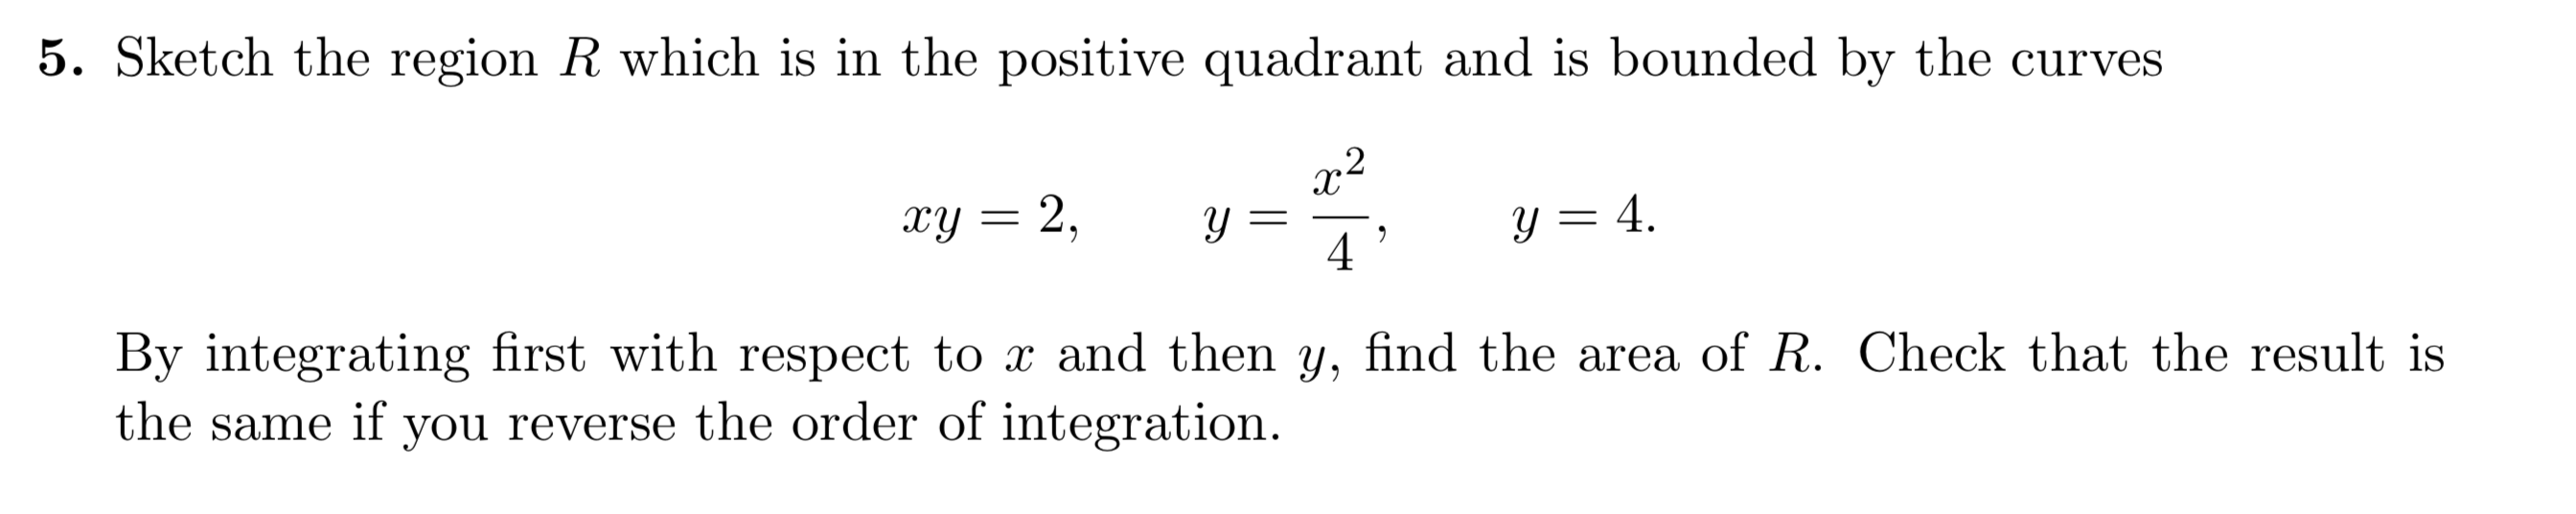
\includegraphics[width=400pt]{img/oxford-prelims-M5-multivariable-calc-1-5.png}
\end{mdframed}

\subsection{}
\begin{mdframed}
  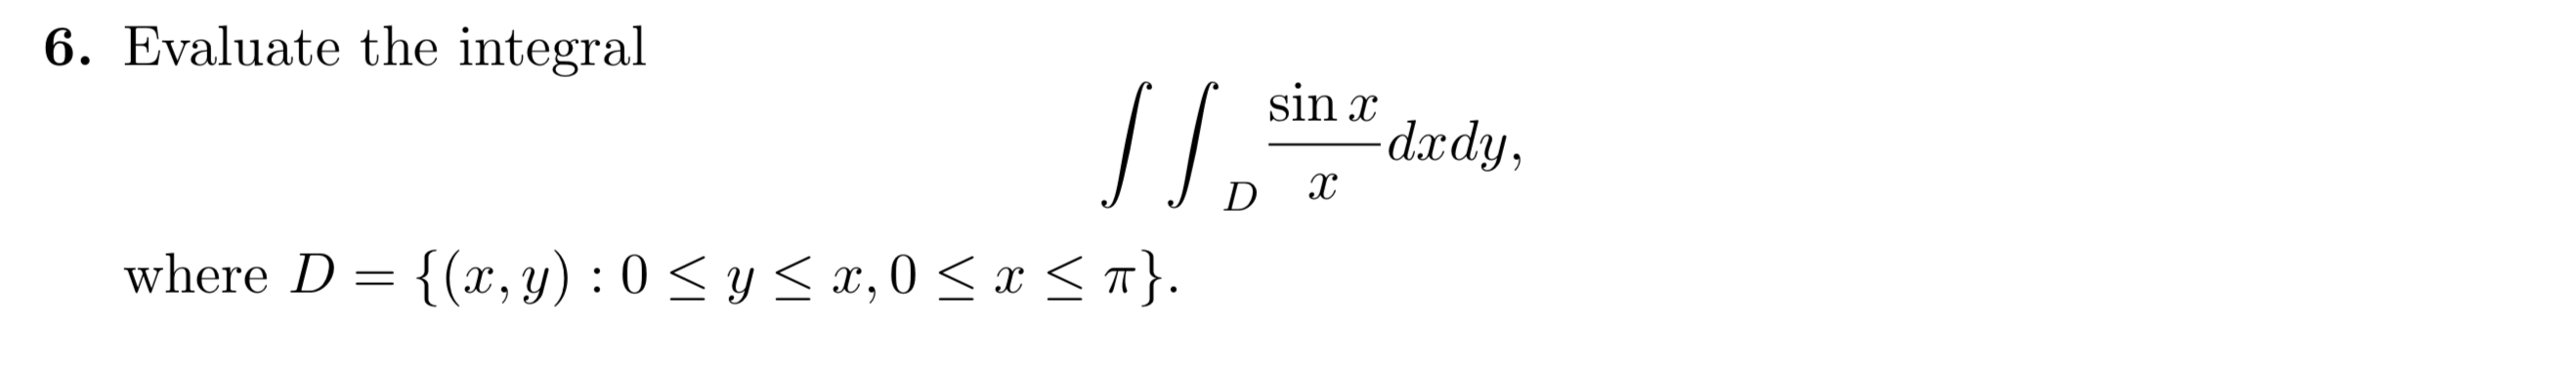
\includegraphics[width=400pt]{img/oxford-prelims-M5-multivariable-calc-1-6.png}
\end{mdframed}

\subsection{}
\begin{mdframed}
  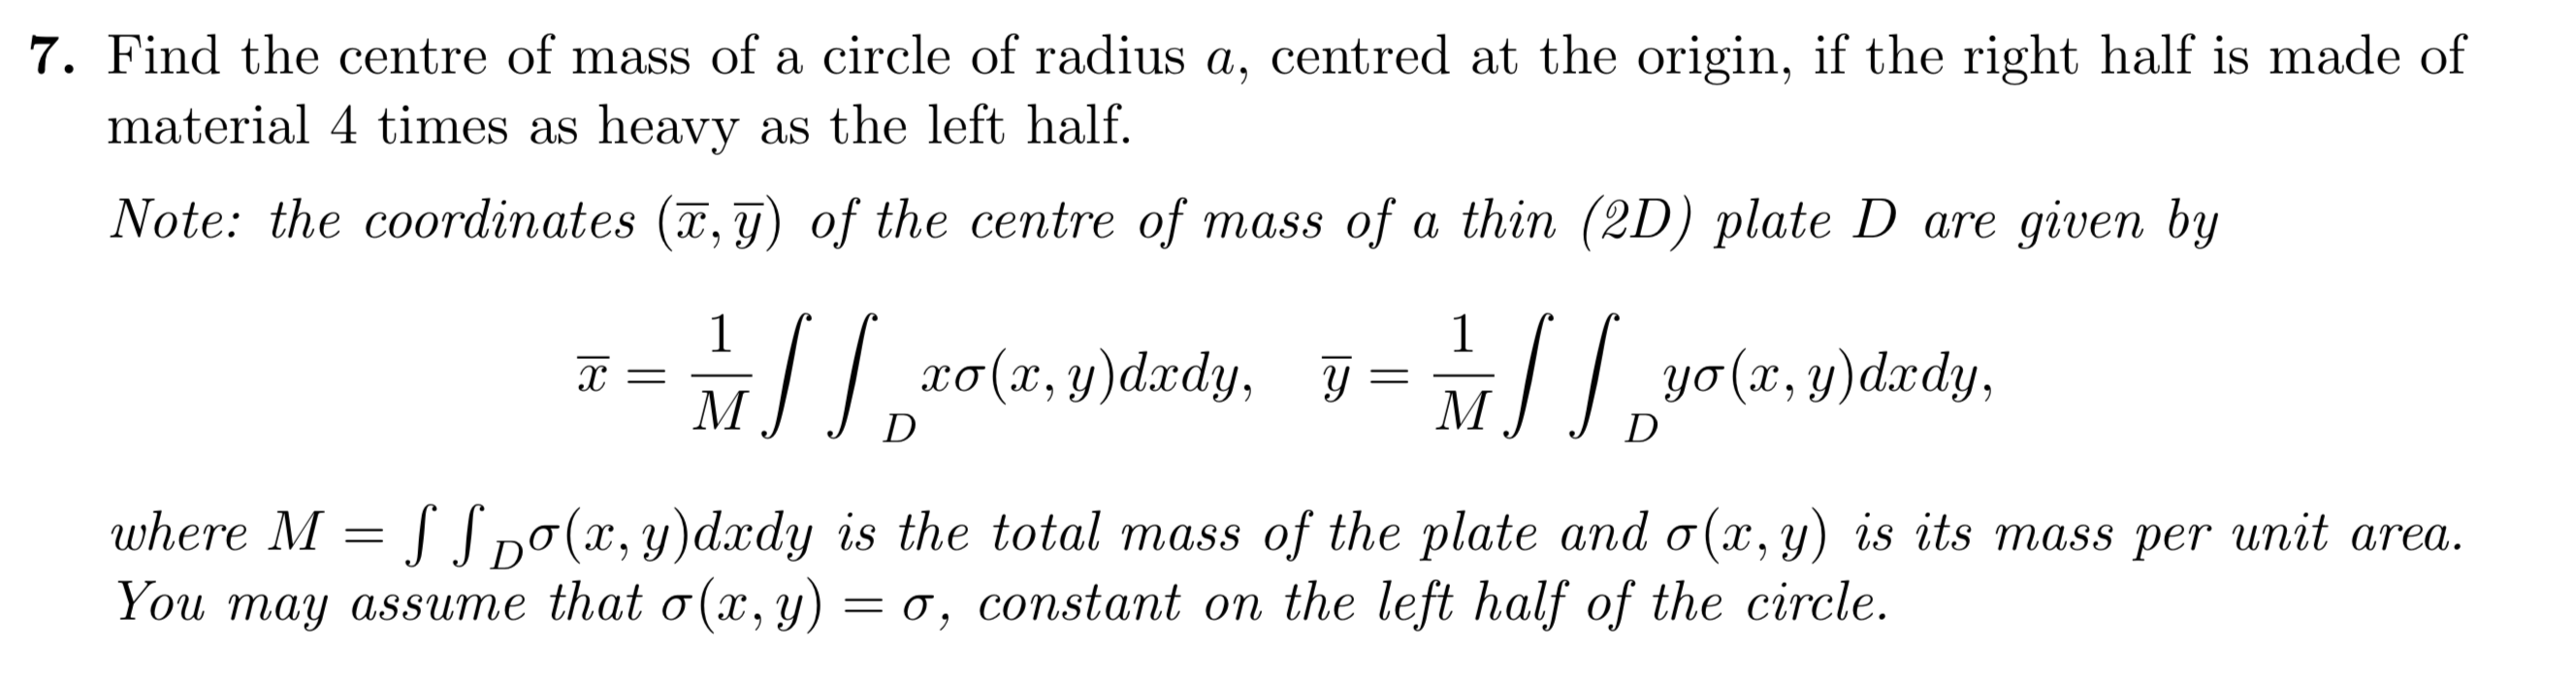
\includegraphics[width=400pt]{img/oxford-prelims-M5-multivariable-calc-1-7.png}
\end{mdframed}


\newpage
\section{Sheet 2}

\subsection{}
\begin{mdframed}
  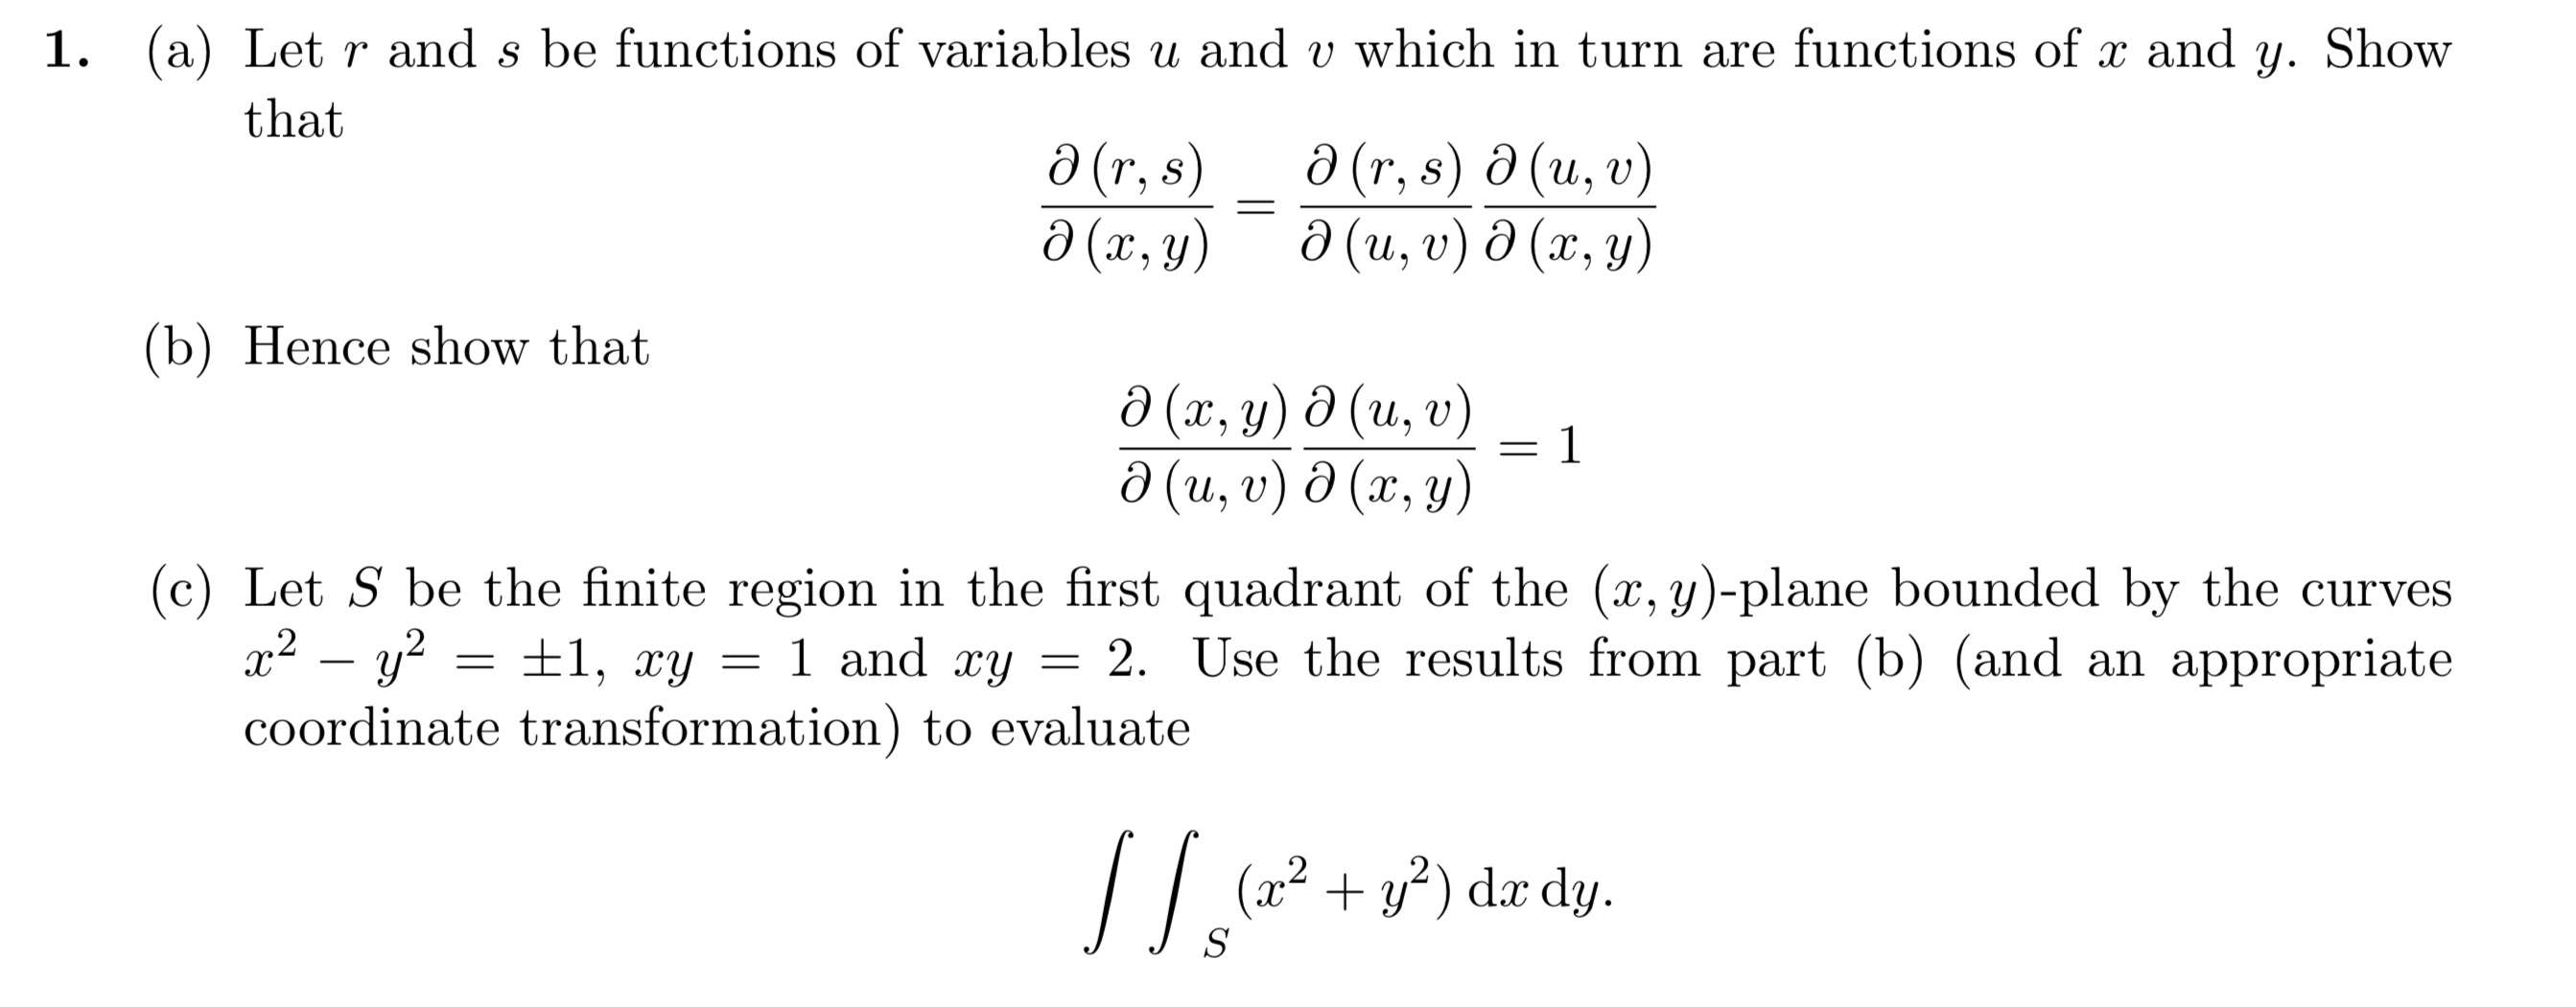
\includegraphics[width=400pt]{img/oxford-prelims-M5-multivariable-calc-2-1.png}
\end{mdframed}

\subsection{}
\begin{mdframed}
  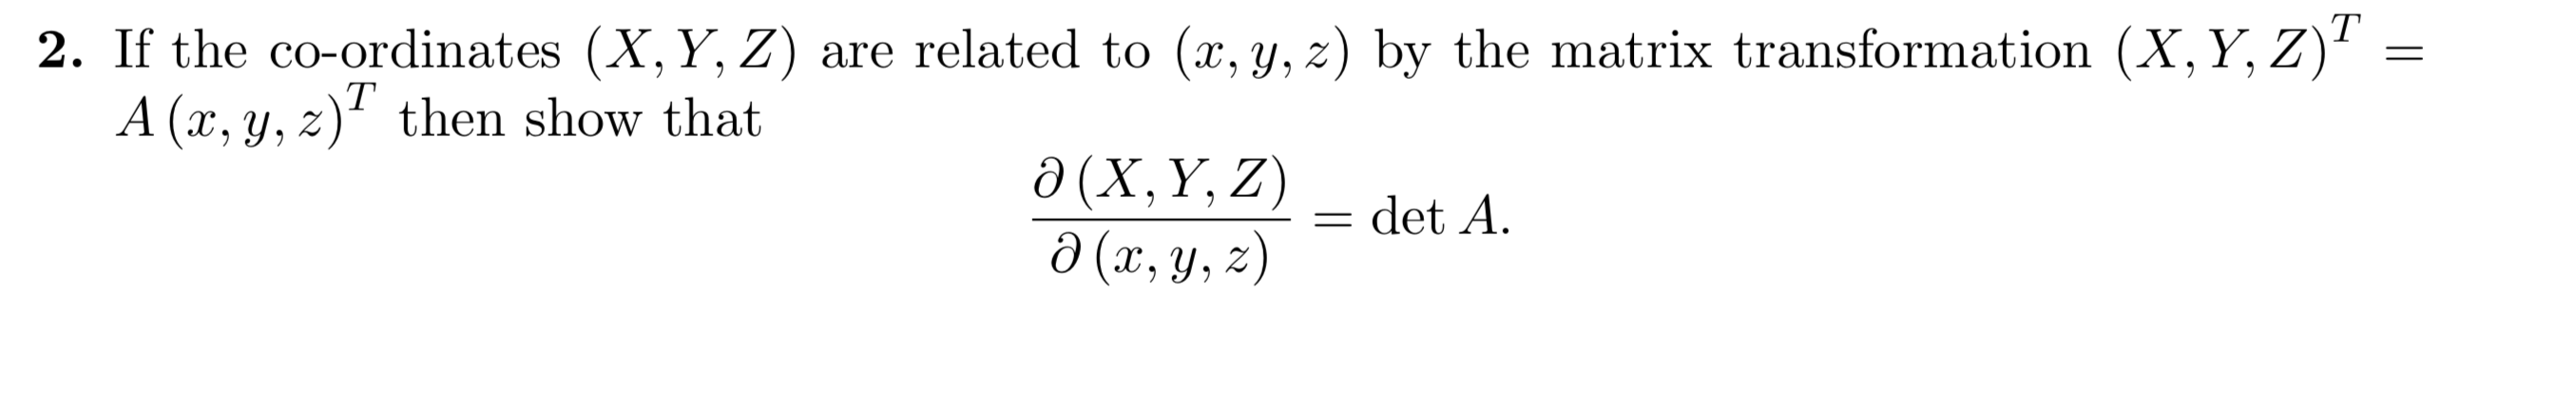
\includegraphics[width=400pt]{img/oxford-prelims-M5-multivariable-calc-2-2.png}
\end{mdframed}

\subsection{}
\begin{mdframed}
  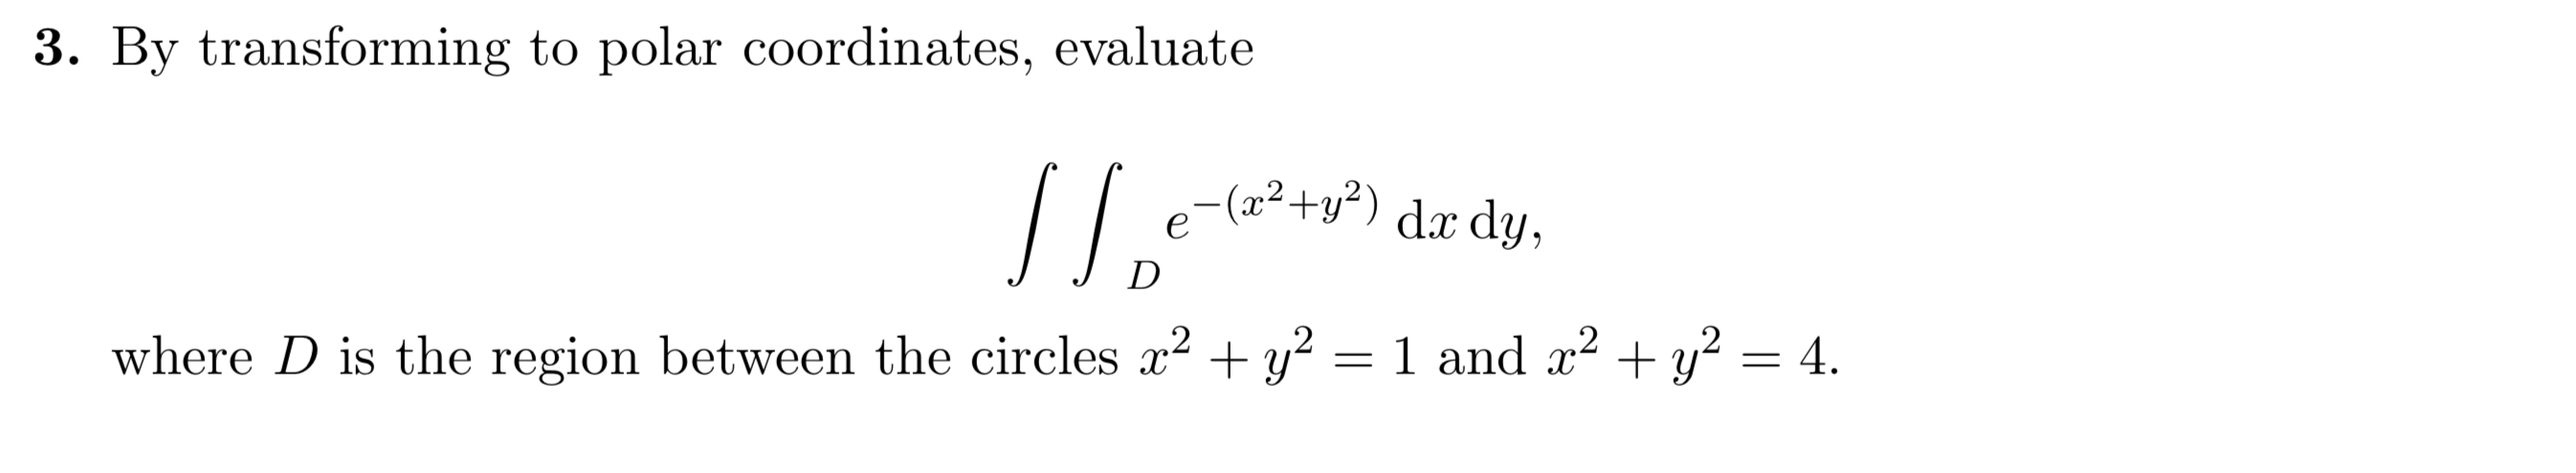
\includegraphics[width=400pt]{img/oxford-prelims-M5-multivariable-calc-2-3.png}
\end{mdframed}

\subsection{}
\begin{mdframed}
  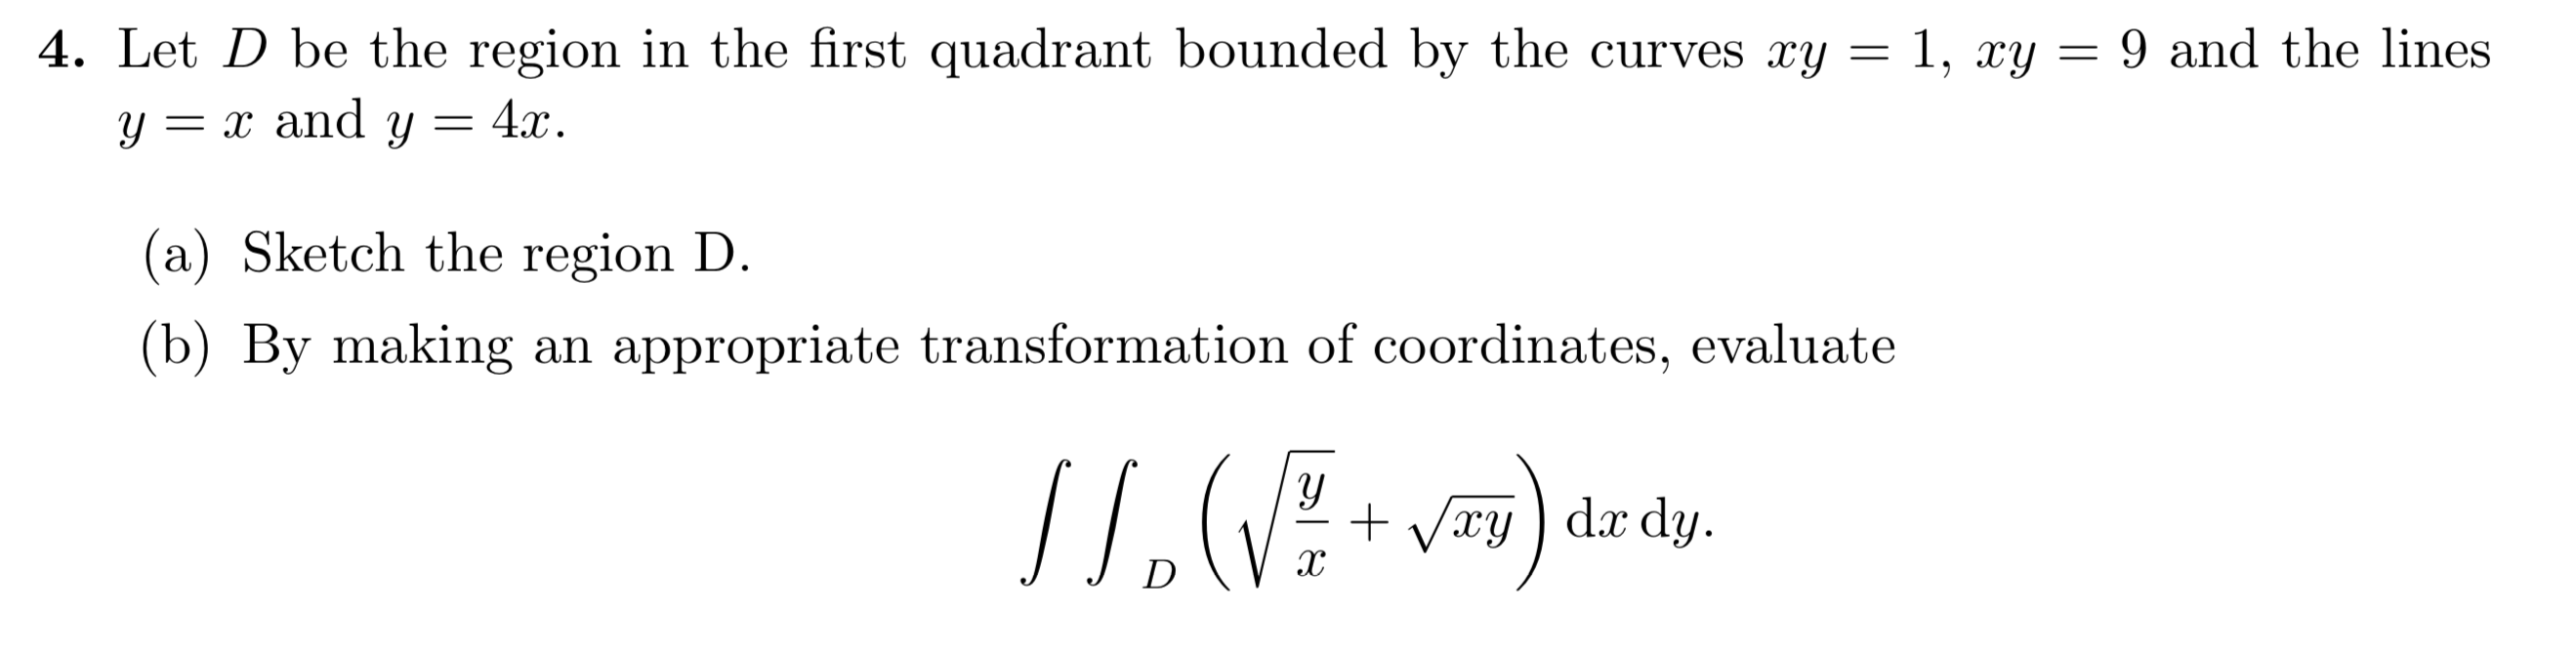
\includegraphics[width=400pt]{img/oxford-prelims-M5-multivariable-calc-2-4.png}
\end{mdframed}

\subsection{}
\begin{mdframed}
  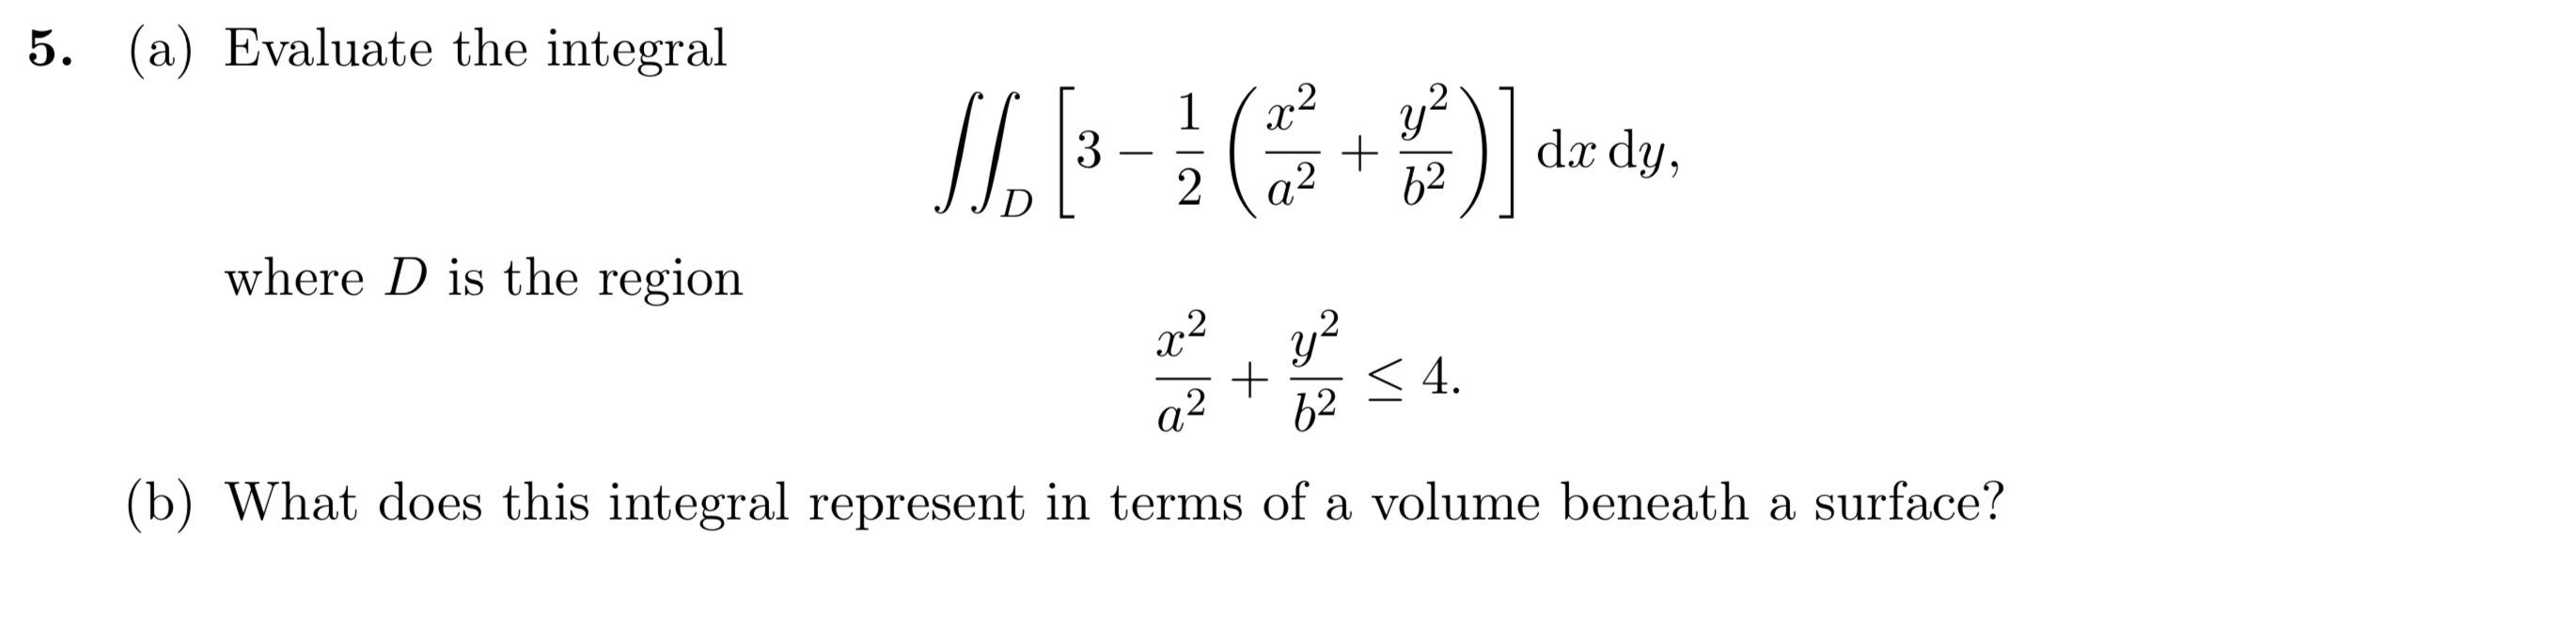
\includegraphics[width=400pt]{img/oxford-prelims-M5-multivariable-calc-2-5.png}
\end{mdframed}



\newpage
\section{Sheet 3}


\subsection{}
\begin{mdframed}
  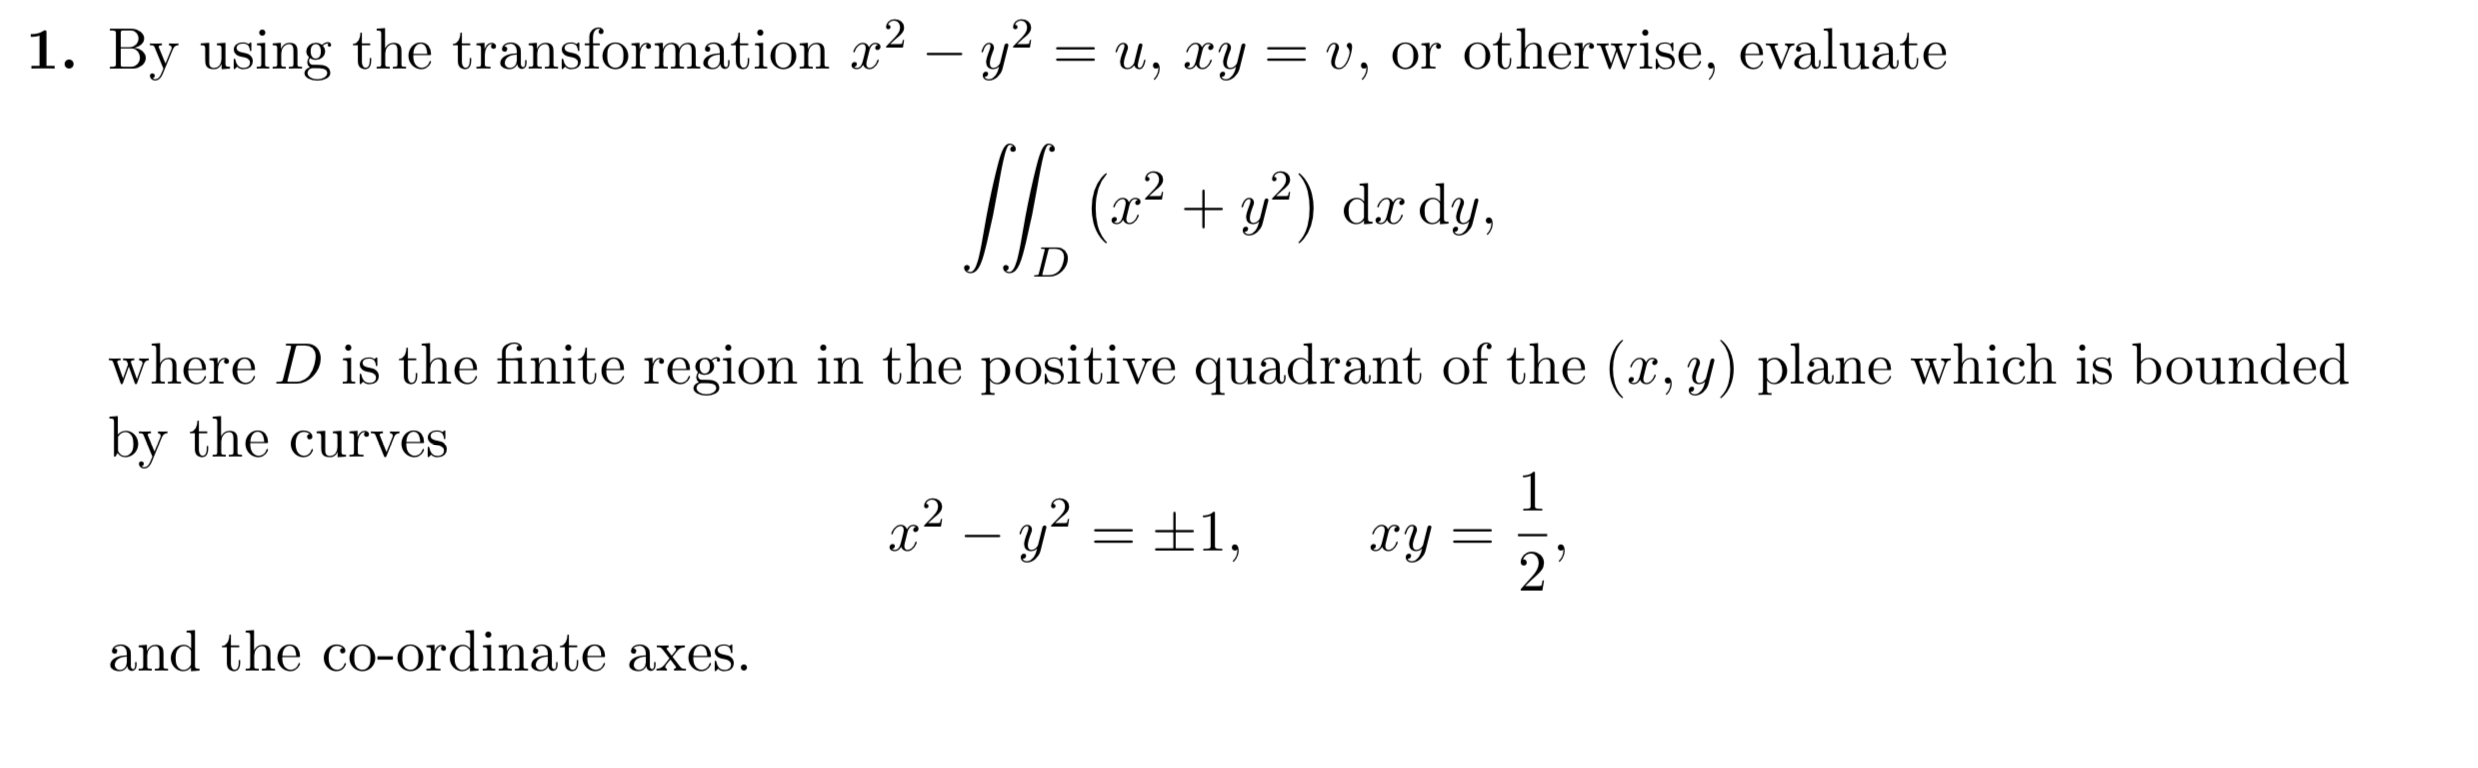
\includegraphics[width=400pt]{img/oxford-prelims-M5-multivariable-calc-3-1.png}
\end{mdframed}

\subsection{}
\begin{mdframed}
  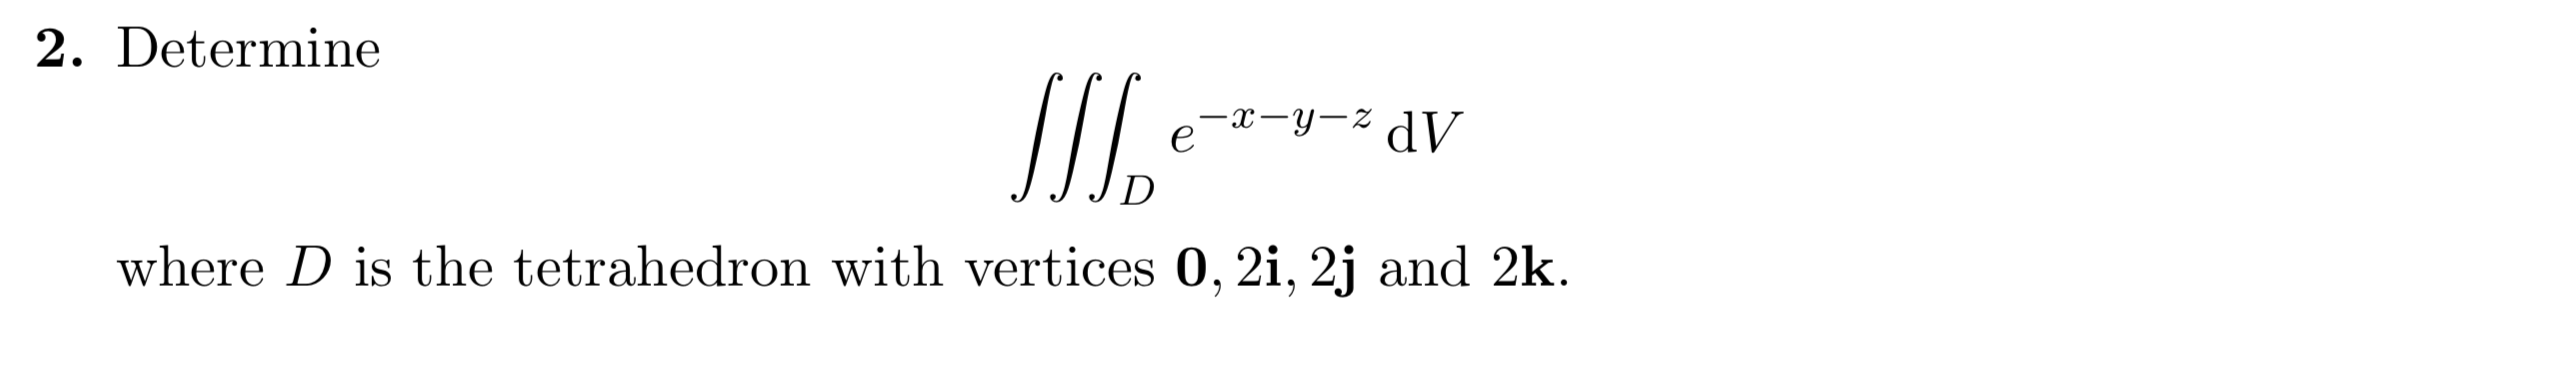
\includegraphics[width=400pt]{img/oxford-prelims-M5-multivariable-calc-3-2.png}
\end{mdframed}

\subsection{}
\begin{mdframed}
  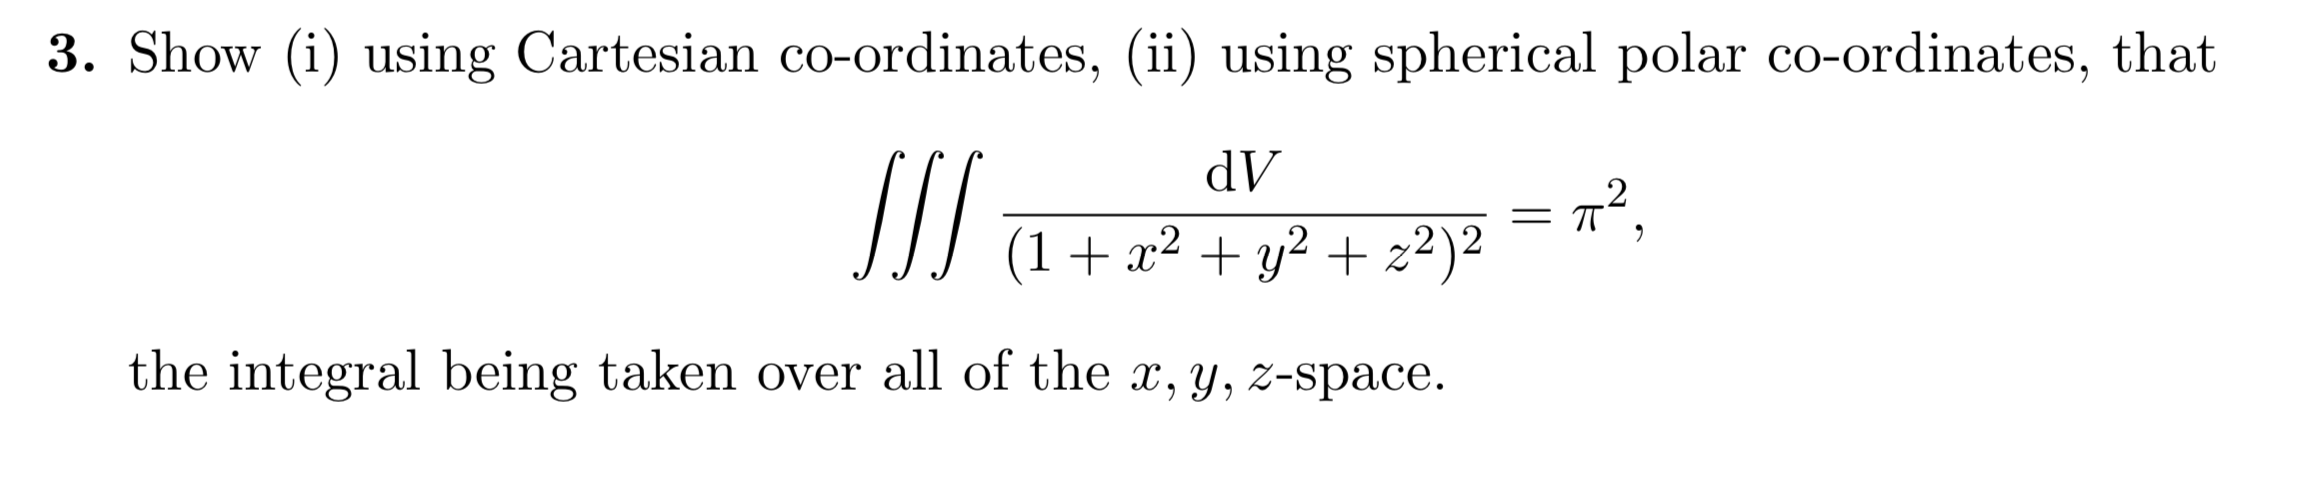
\includegraphics[width=400pt]{img/oxford-prelims-M5-multivariable-calc-3-3.png}
\end{mdframed}

\subsection{}
\begin{mdframed}
  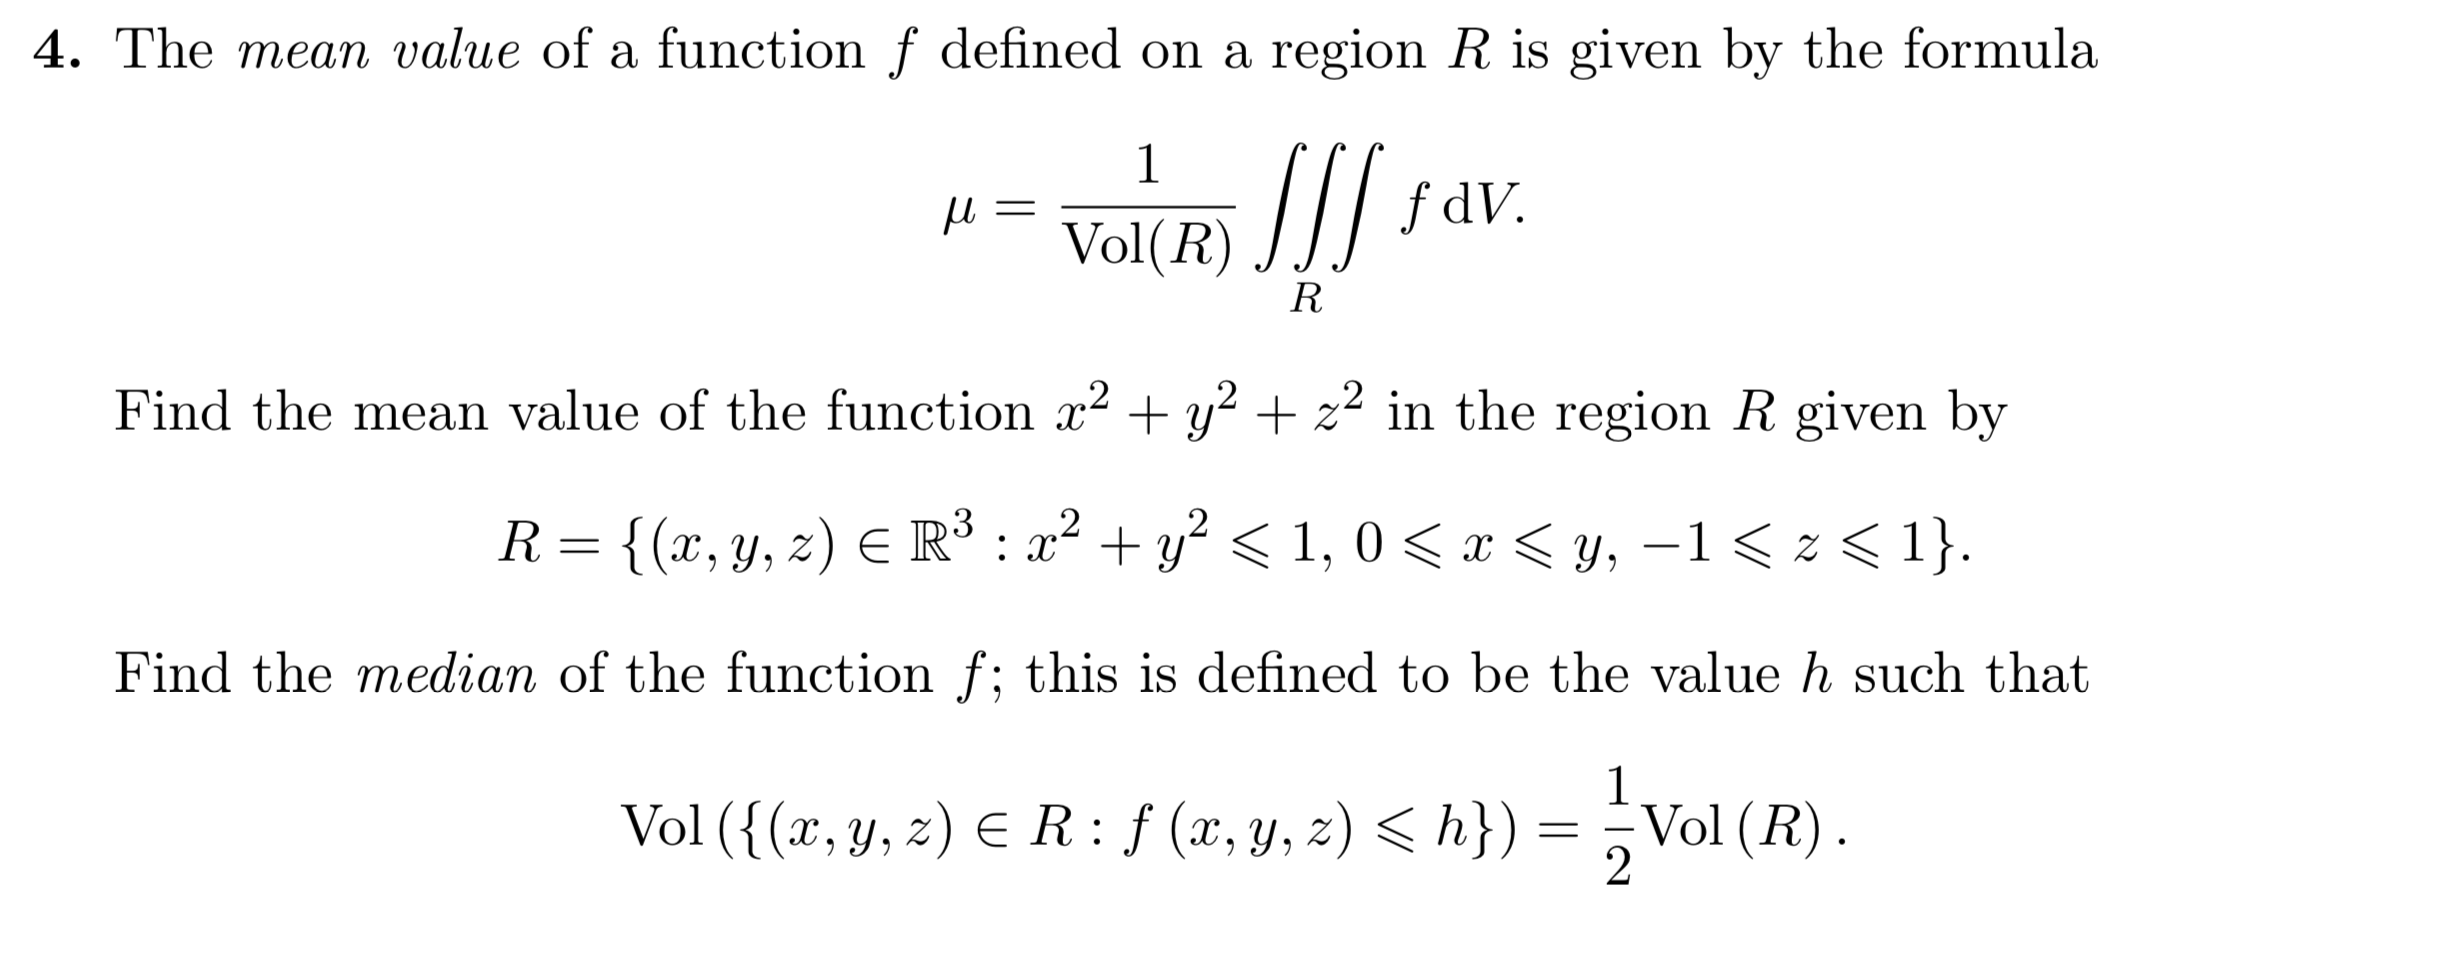
\includegraphics[width=400pt]{img/oxford-prelims-M5-multivariable-calc-3-4.png}
\end{mdframed}

\subsection{}
\begin{mdframed}
  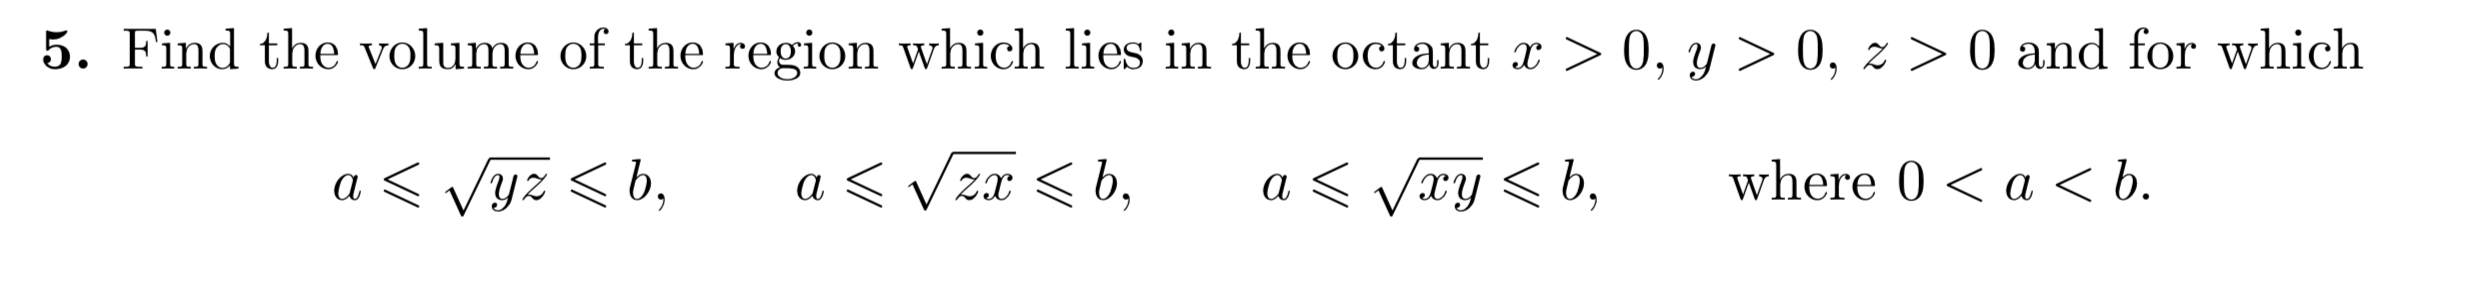
\includegraphics[width=400pt]{img/oxford-prelims-M5-multivariable-calc-3-5.png}
\end{mdframed}


\newpage
\section{Sheet 4}

\subsection{}
\begin{mdframed}
  
\includegraphics[width=400pt]{img/oxford-prelims-M5-multivariable-calc-4-1.png}
\end{mdframed}

\subsection{}
\begin{mdframed}
  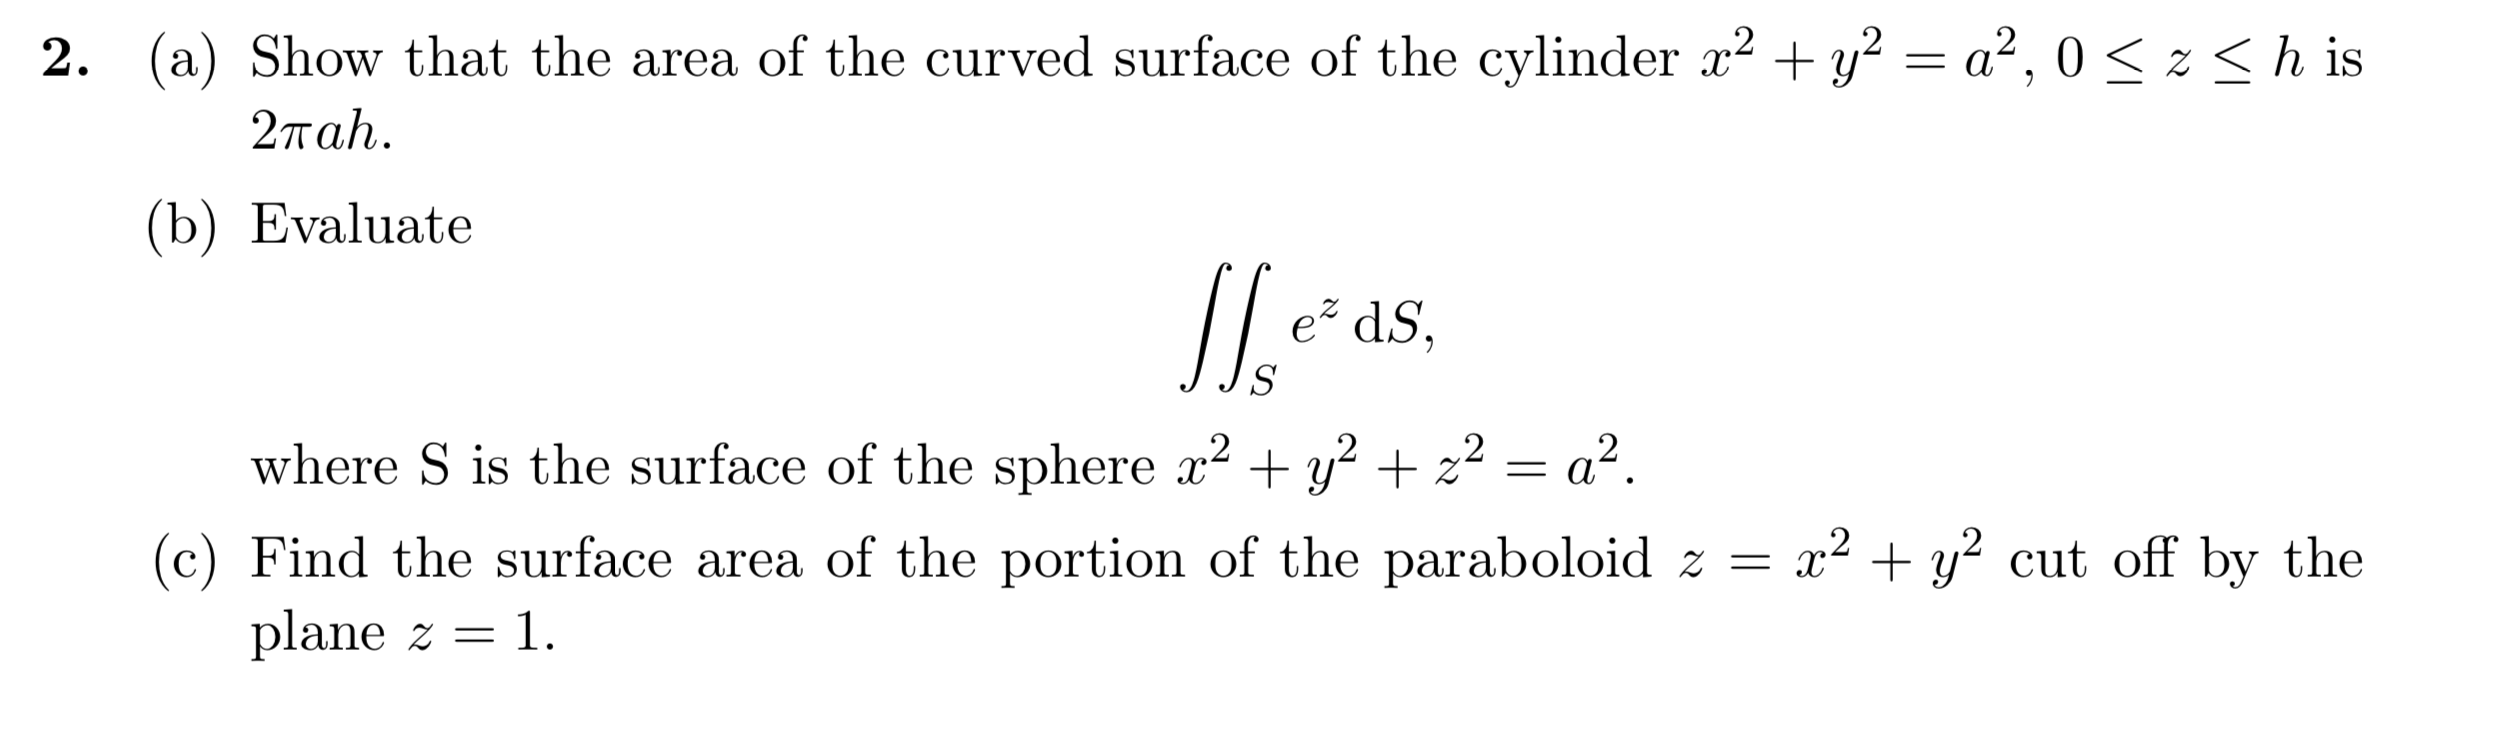
\includegraphics[width=400pt]{img/oxford-prelims-M5-multivariable-calc-4-2.png}
\end{mdframed}

\subsection{}
\begin{mdframed}
  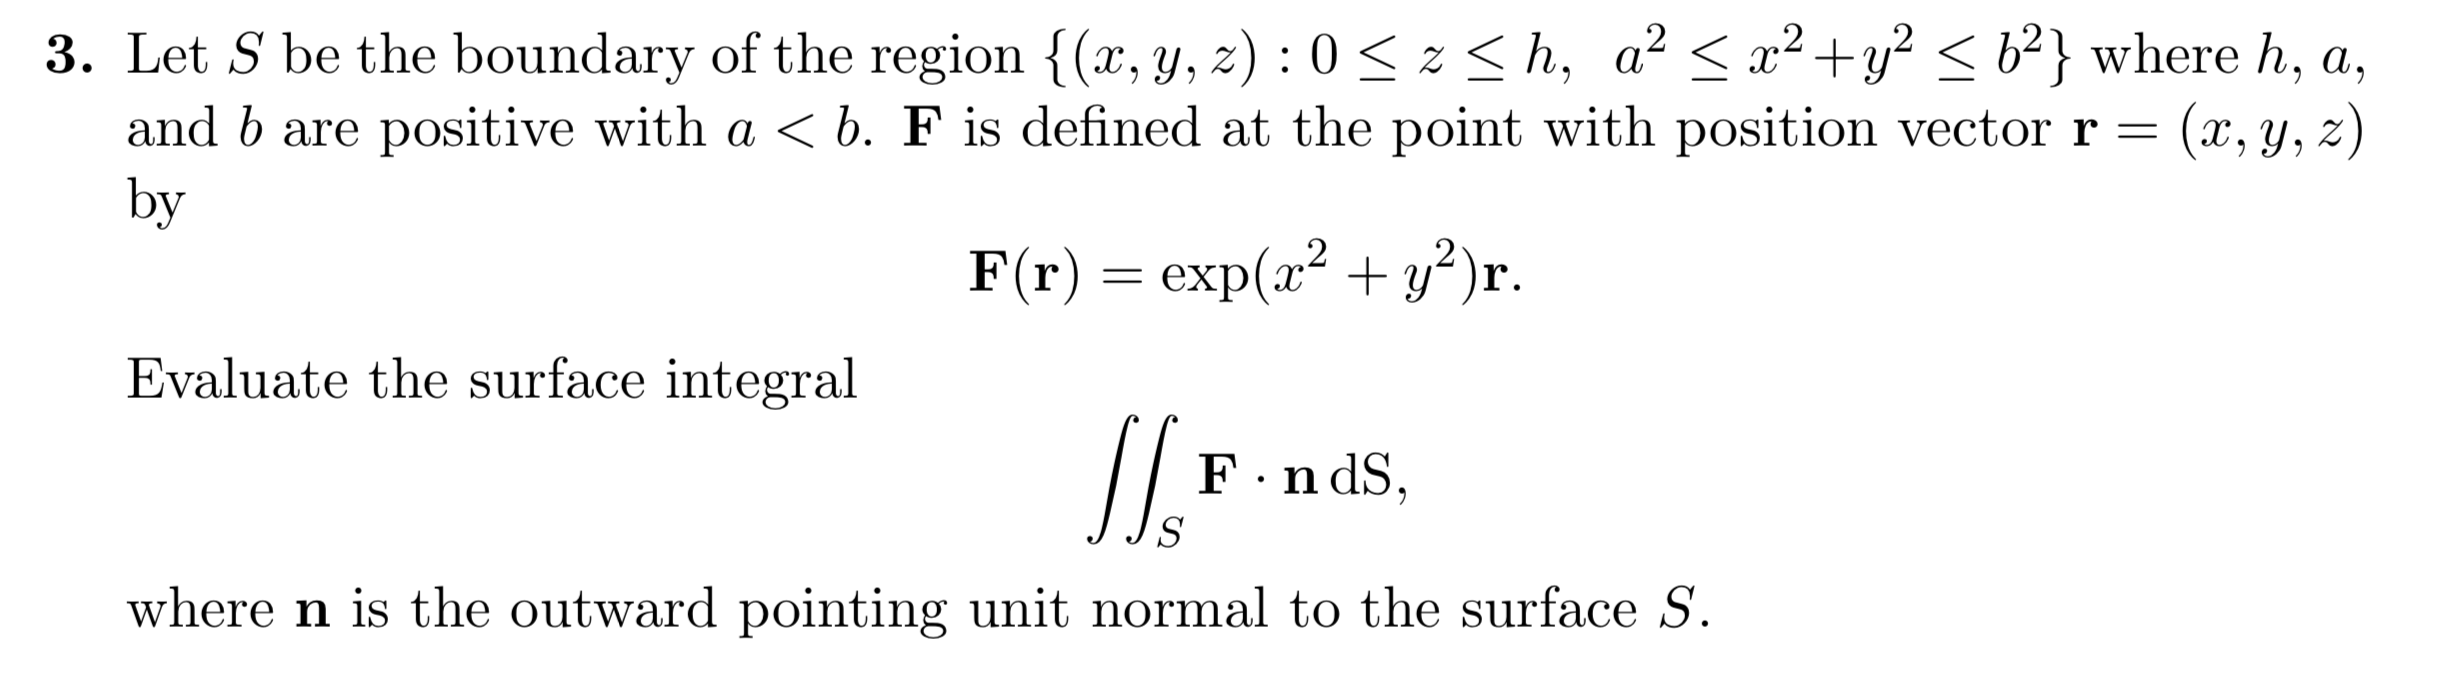
\includegraphics[width=400pt]{img/oxford-prelims-M5-multivariable-calc-4-3.png}
\end{mdframed}

\subsection{}
\begin{mdframed}
  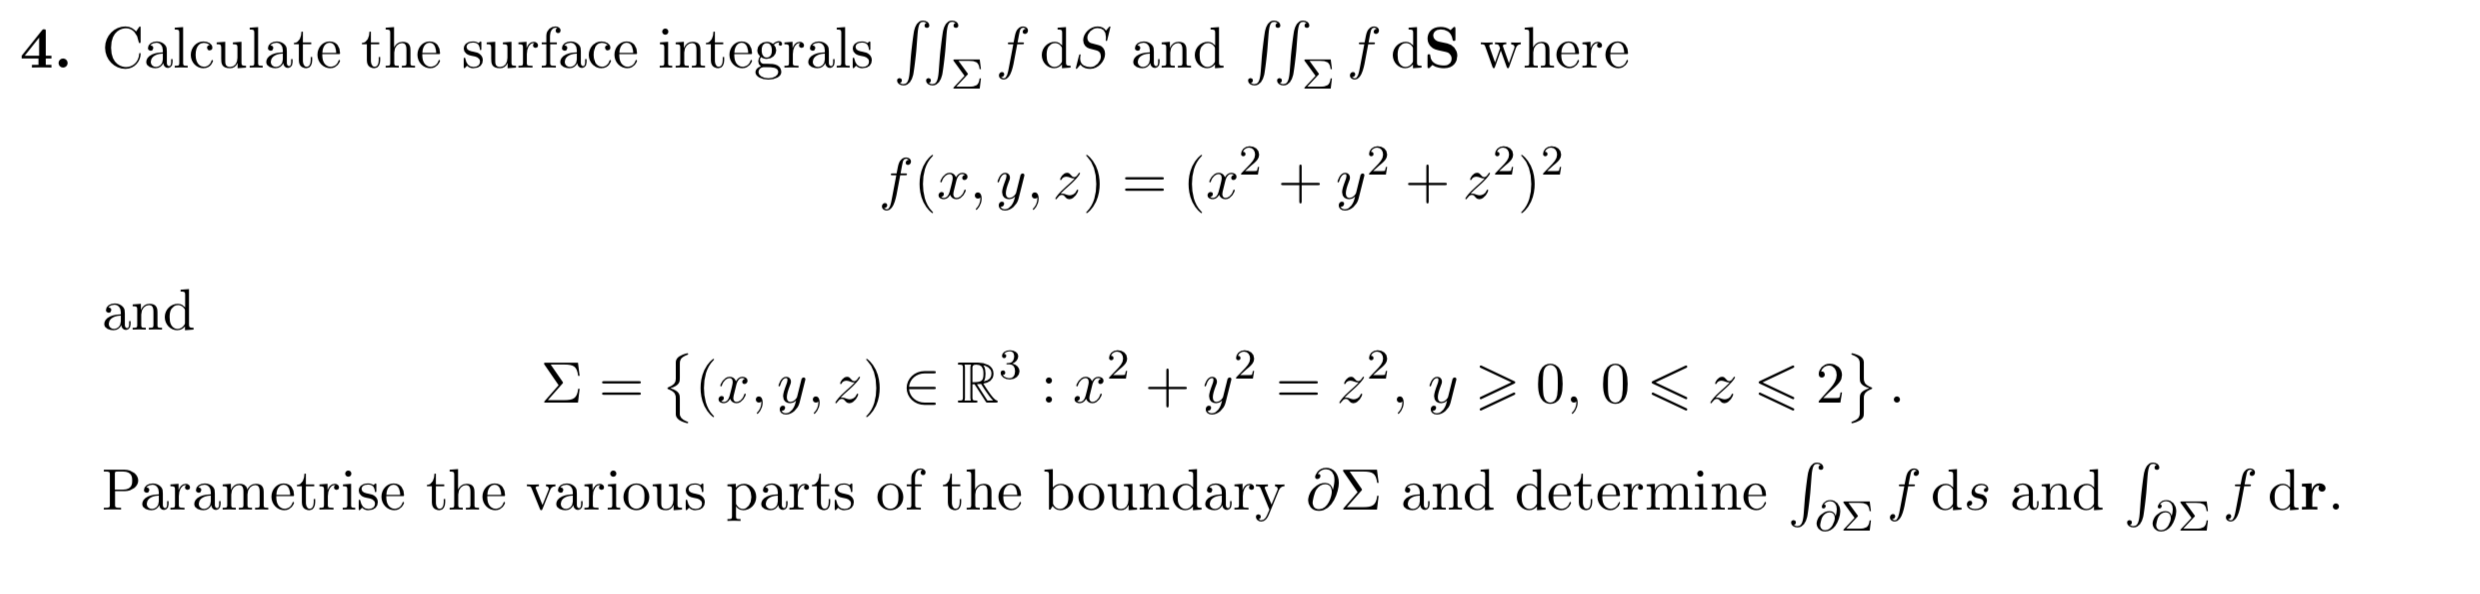
\includegraphics[width=400pt]{img/oxford-prelims-M5-multivariable-calc-4-4.png}
\end{mdframed}

\newpage
\section{Sheet 5}

\subsection{}
\begin{mdframed}
  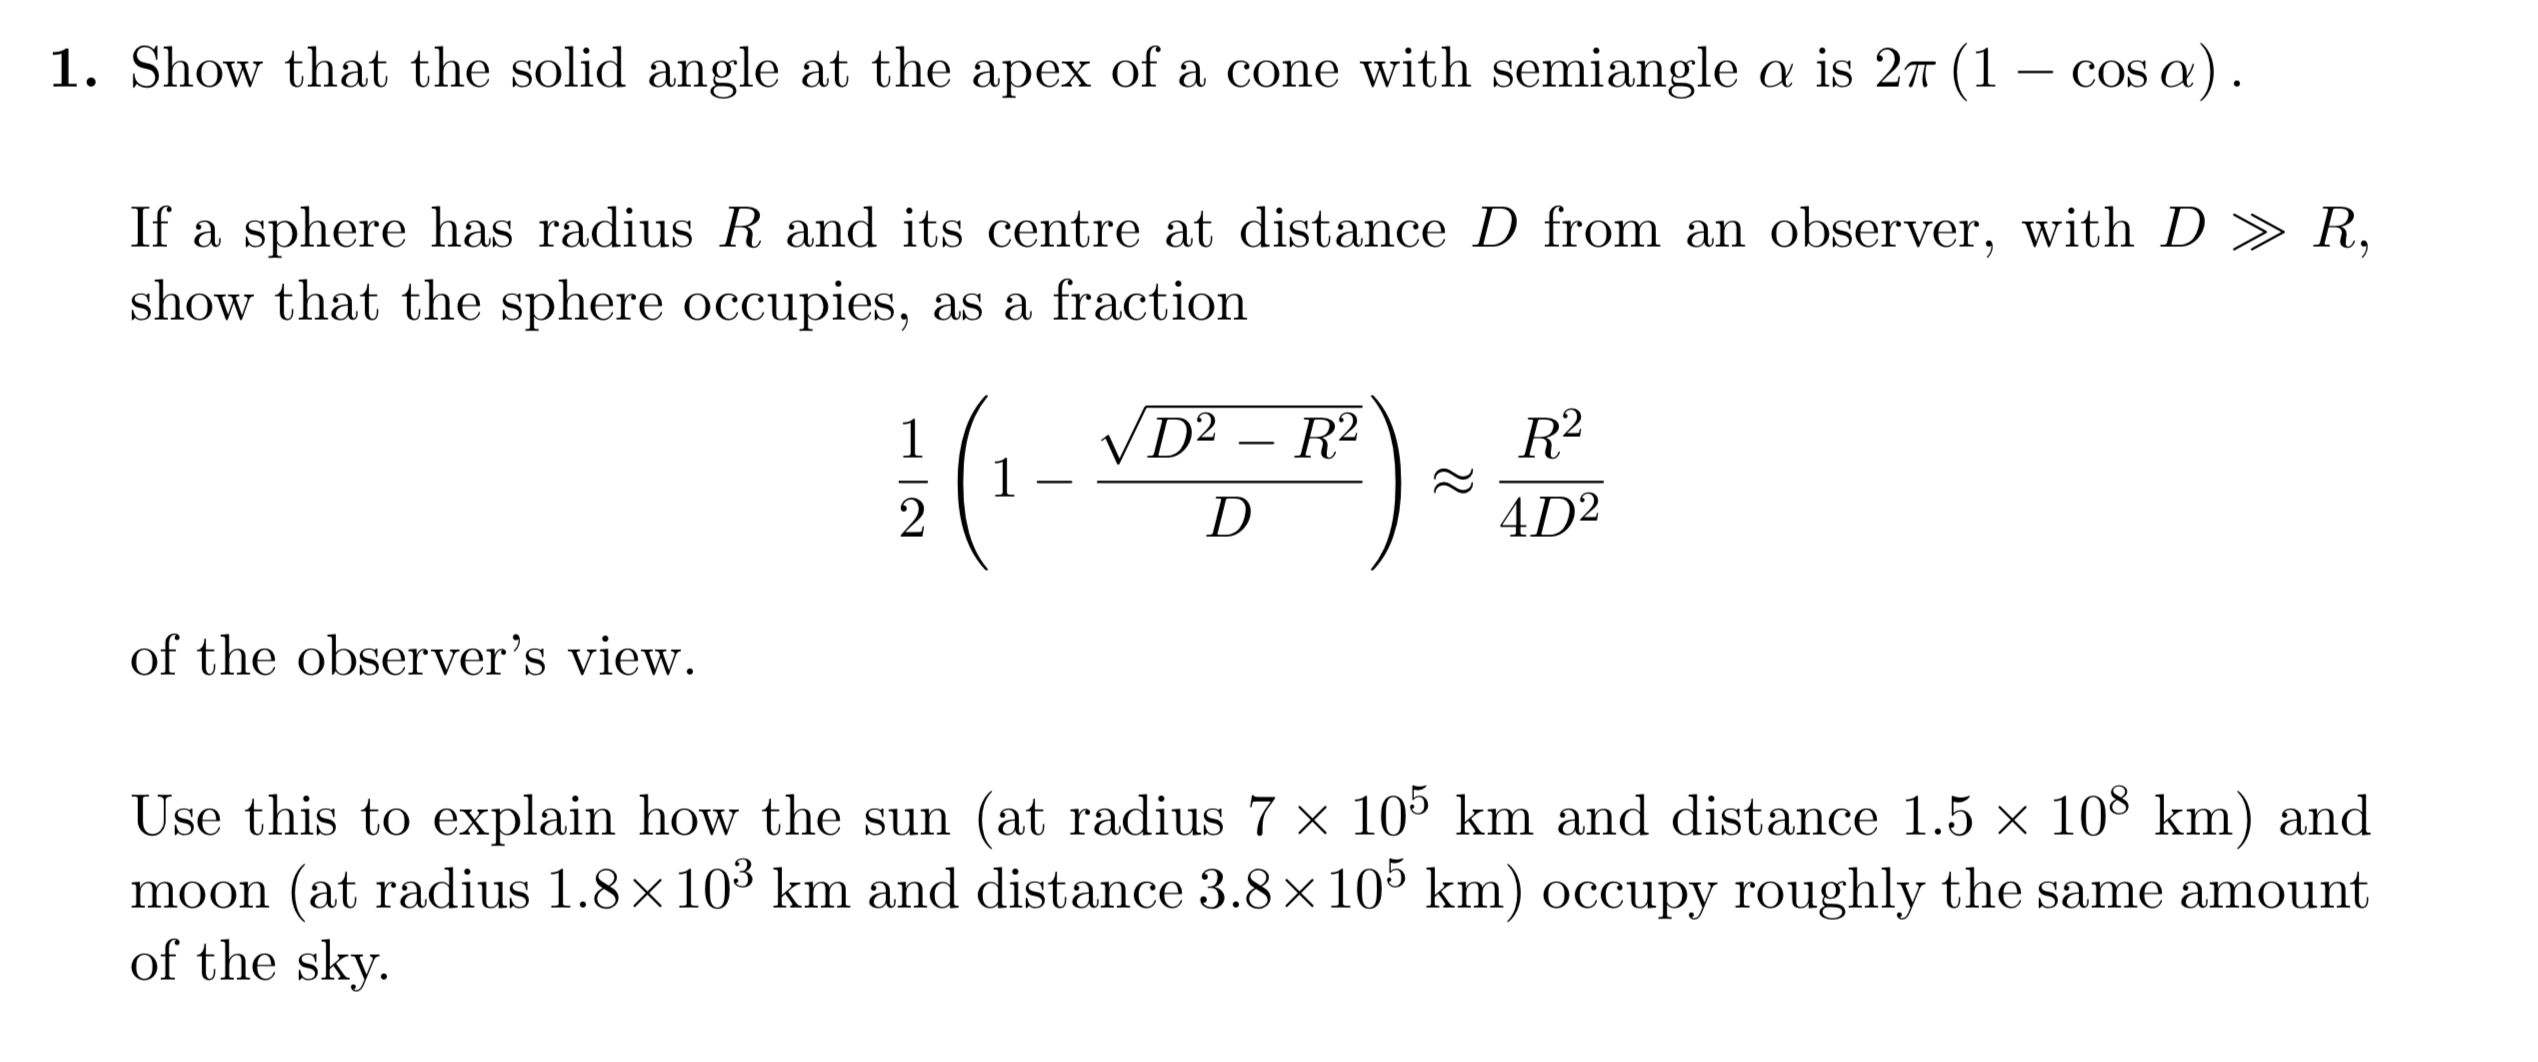
\includegraphics[width=400pt]{img/oxford-prelims-M5-multivariable-calc-5-1.png}
\end{mdframed}

\subsection{}
\begin{mdframed}
  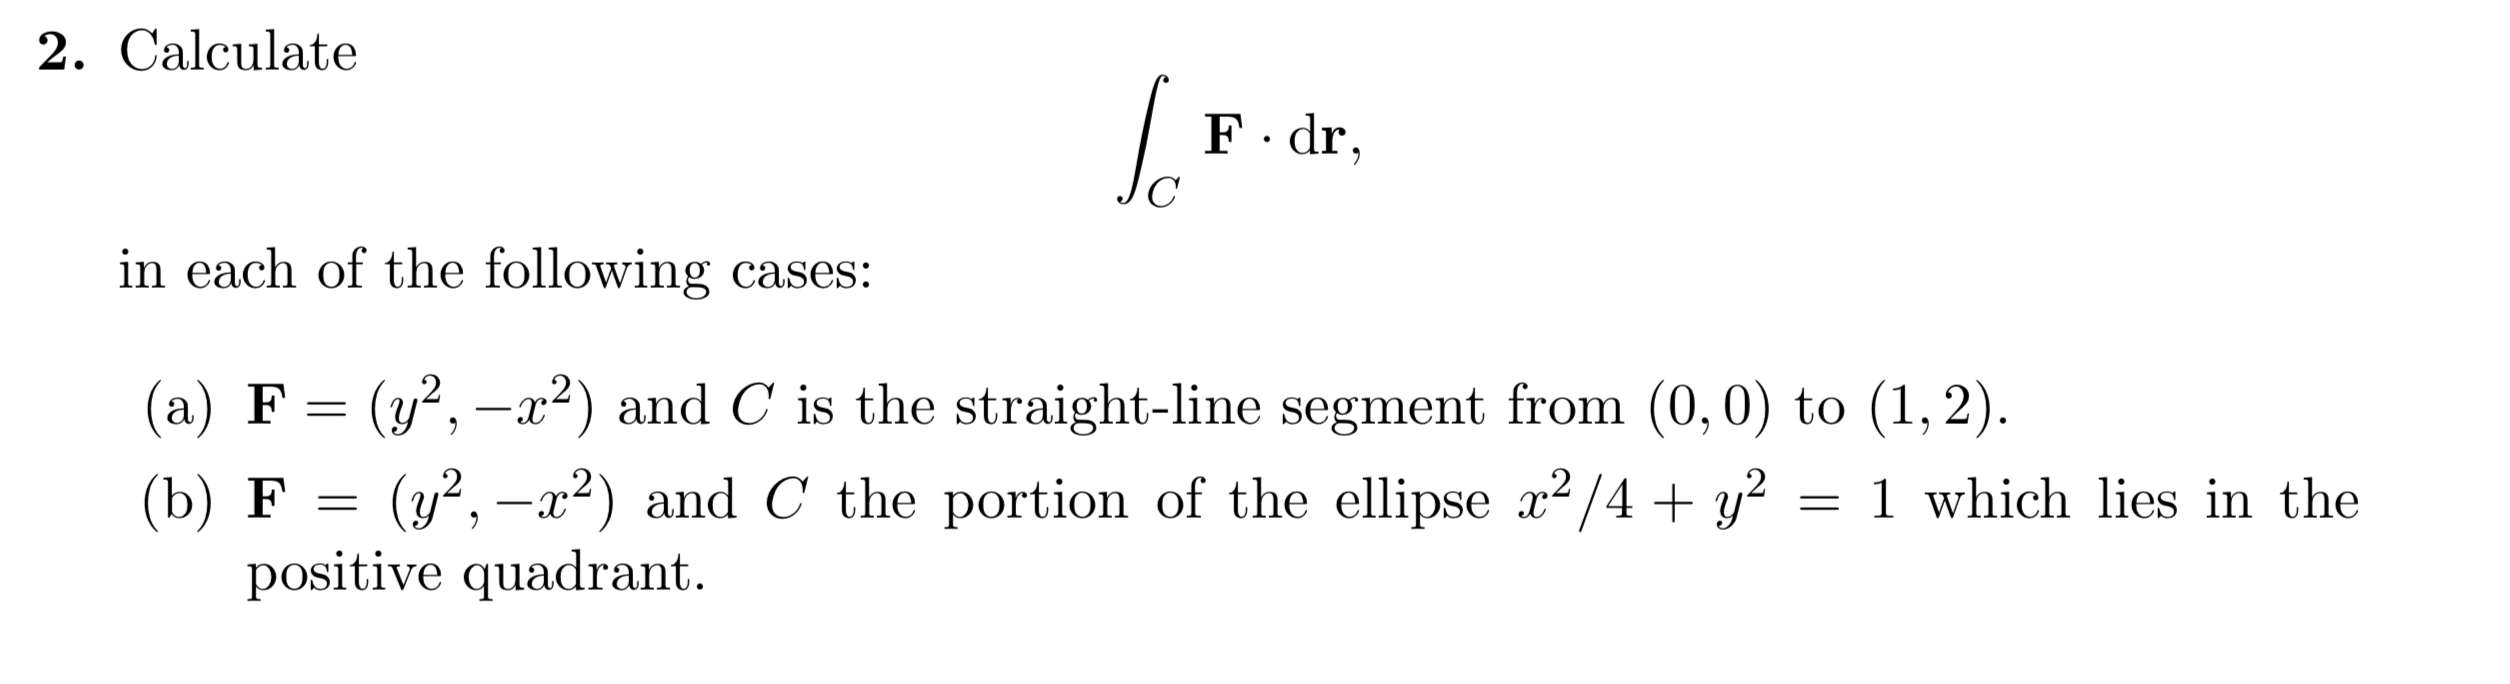
\includegraphics[width=400pt]{img/oxford-prelims-M5-multivariable-calc-5-2.png}
\end{mdframed}

\subsection{}
\begin{mdframed}
  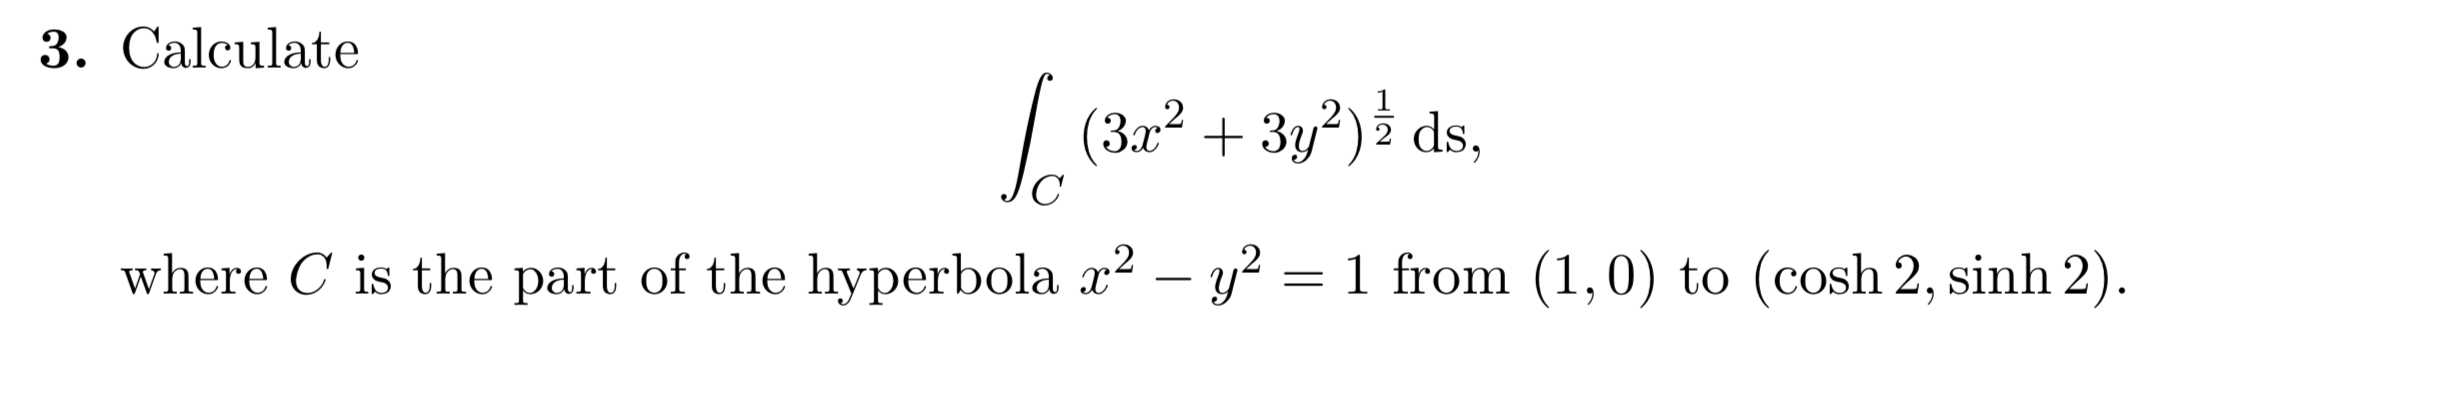
\includegraphics[width=400pt]{img/oxford-prelims-M5-multivariable-calc-5-3.png}
\end{mdframed}

\subsection{}
\begin{mdframed}
  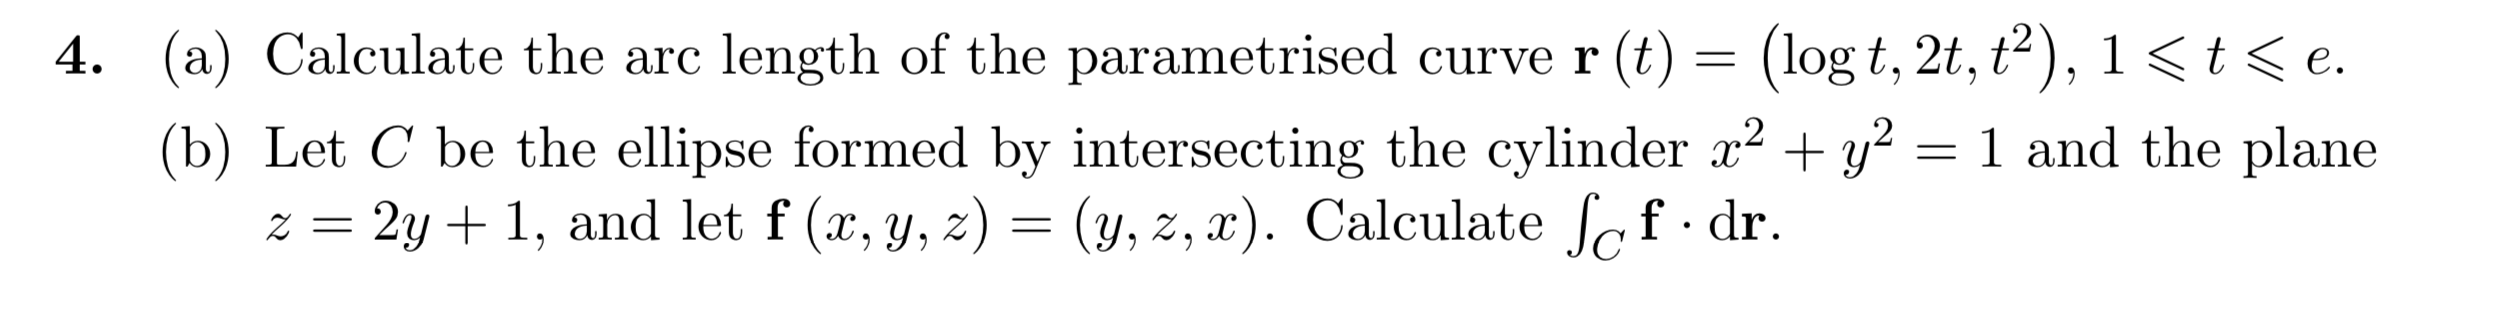
\includegraphics[width=400pt]{img/oxford-prelims-M5-multivariable-calc-5-4.png}
\end{mdframed}

\subsection{}
\begin{mdframed}
  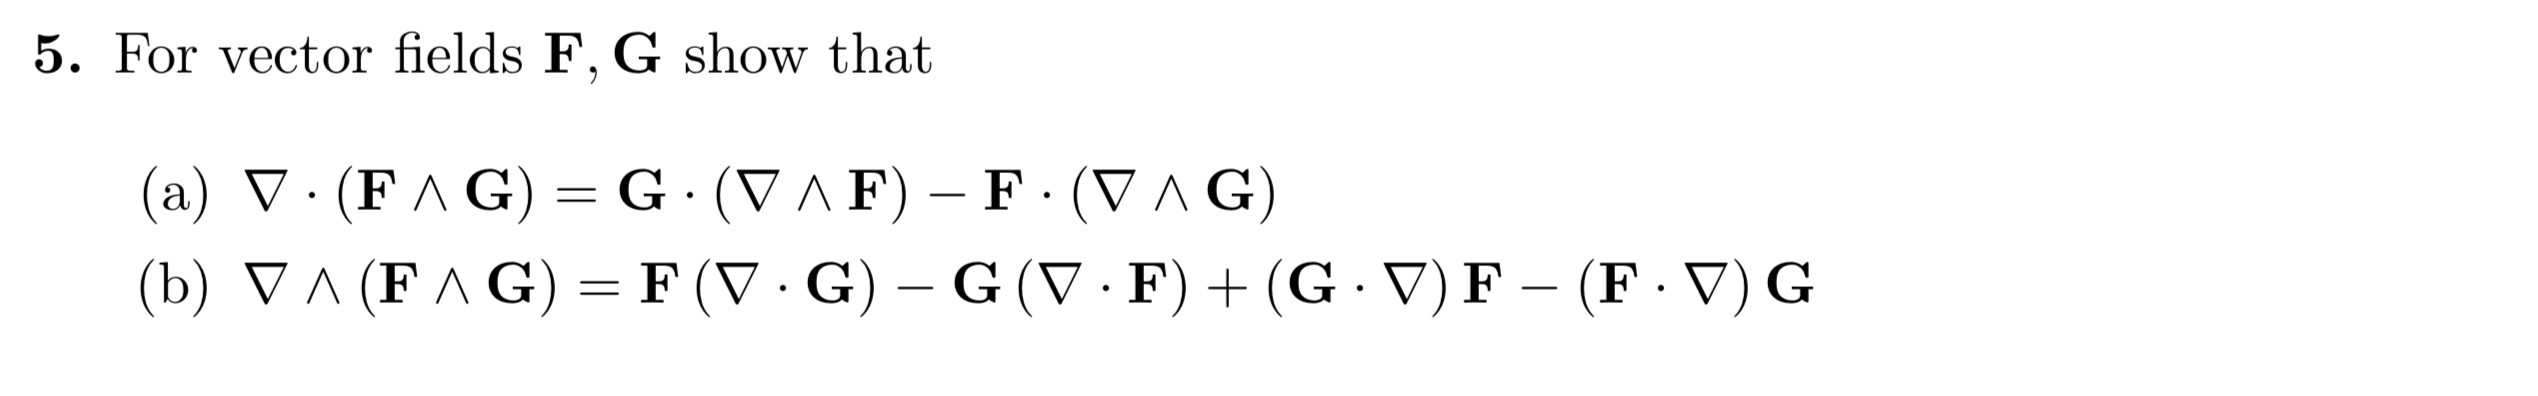
\includegraphics[width=400pt]{img/oxford-prelims-M5-multivariable-calc-5-5.png}
\end{mdframed}


\newpage
\section{Sheet 6}
\begin{mdframed}
  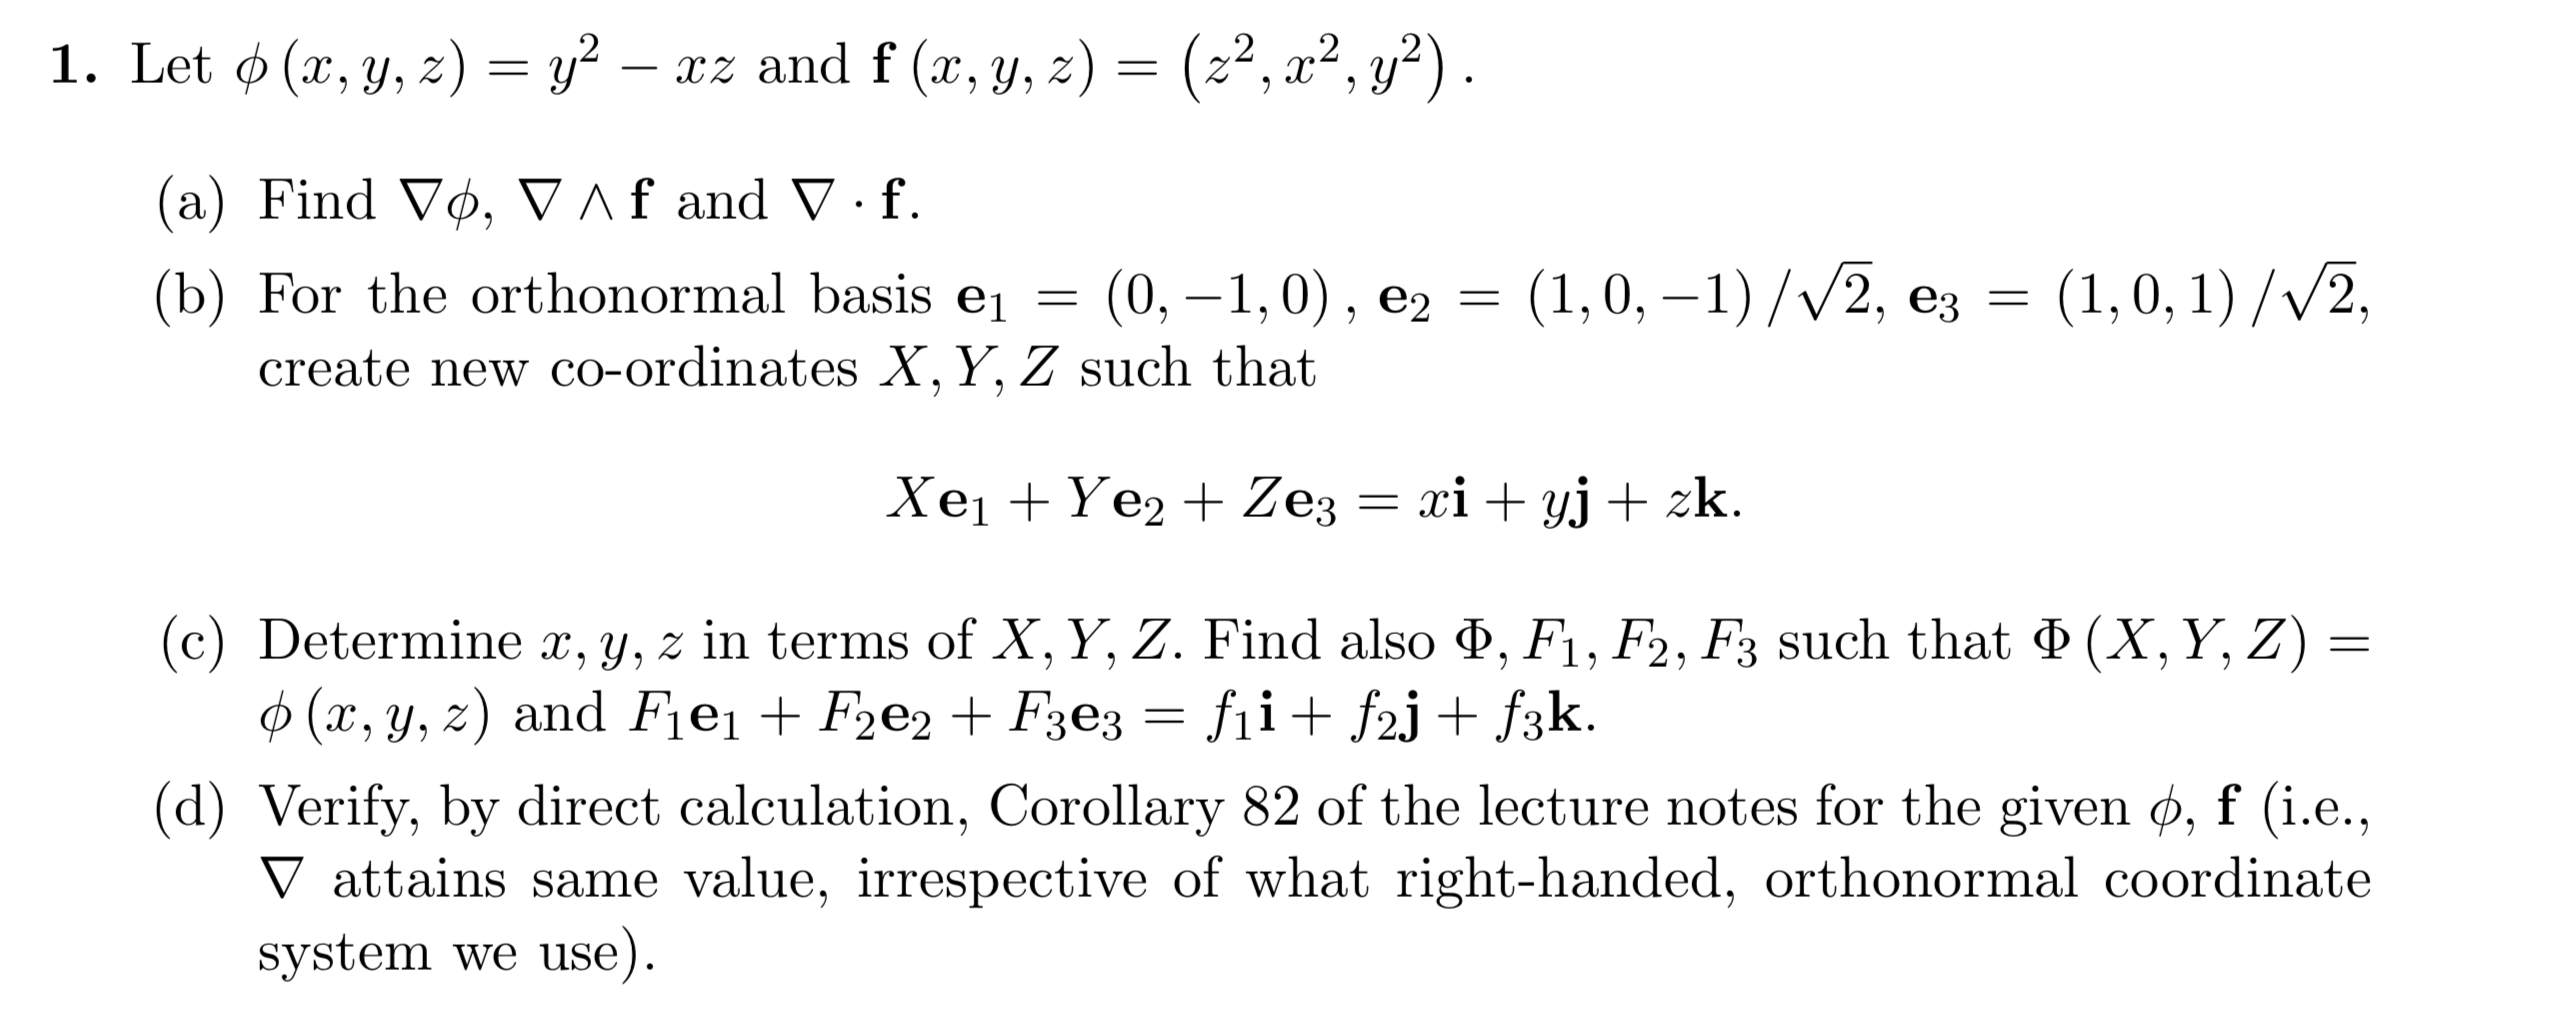
\includegraphics[width=400pt]{img/oxford-prelims-M5-multivariable-calc-6-1.png}
\end{mdframed}

\subsection{}
\begin{mdframed}
  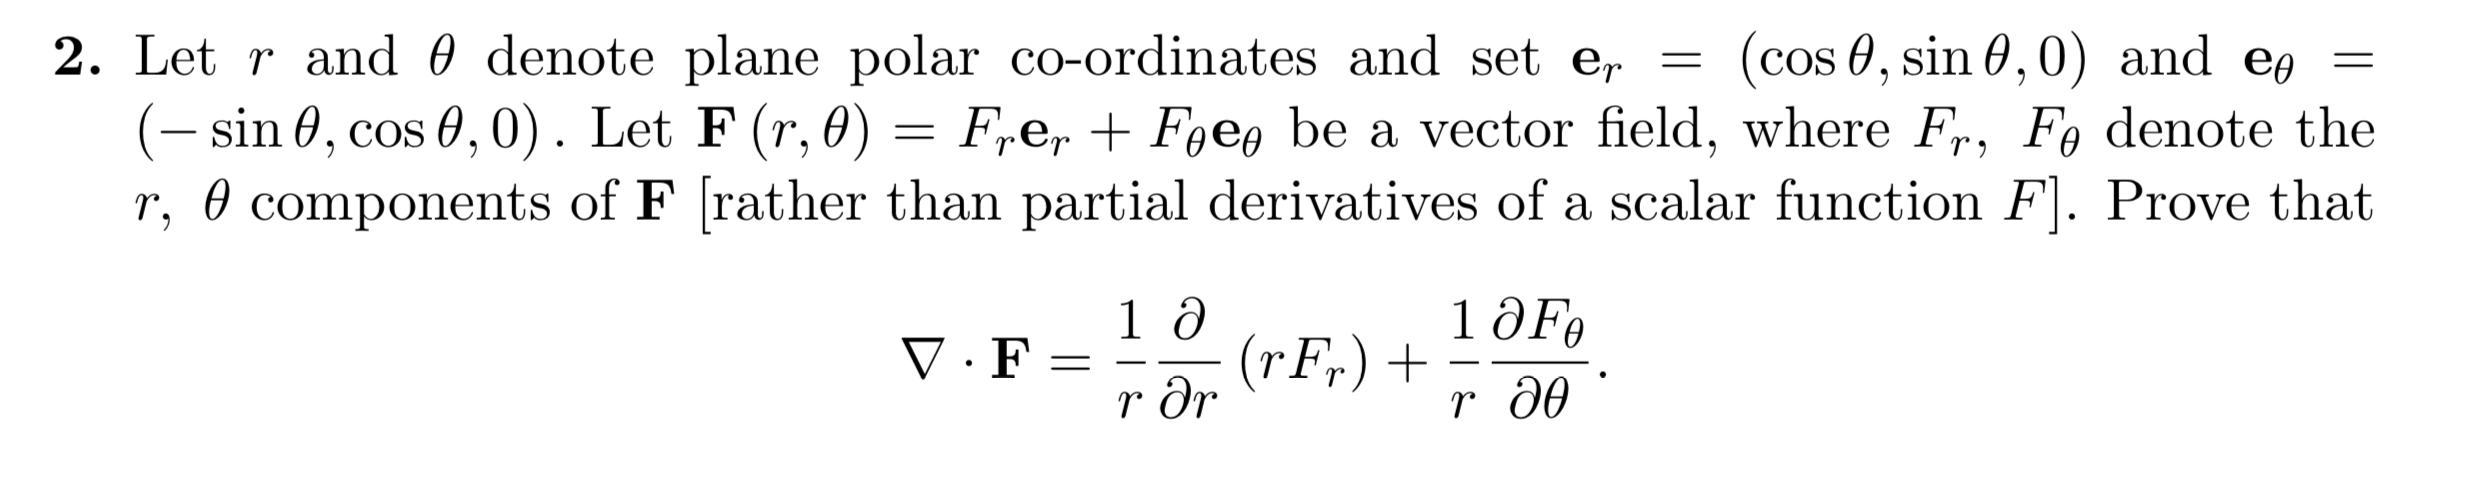
\includegraphics[width=400pt]{img/oxford-prelims-M5-multivariable-calc-6-2.png}
\end{mdframed}

\subsection{}
\begin{mdframed}
  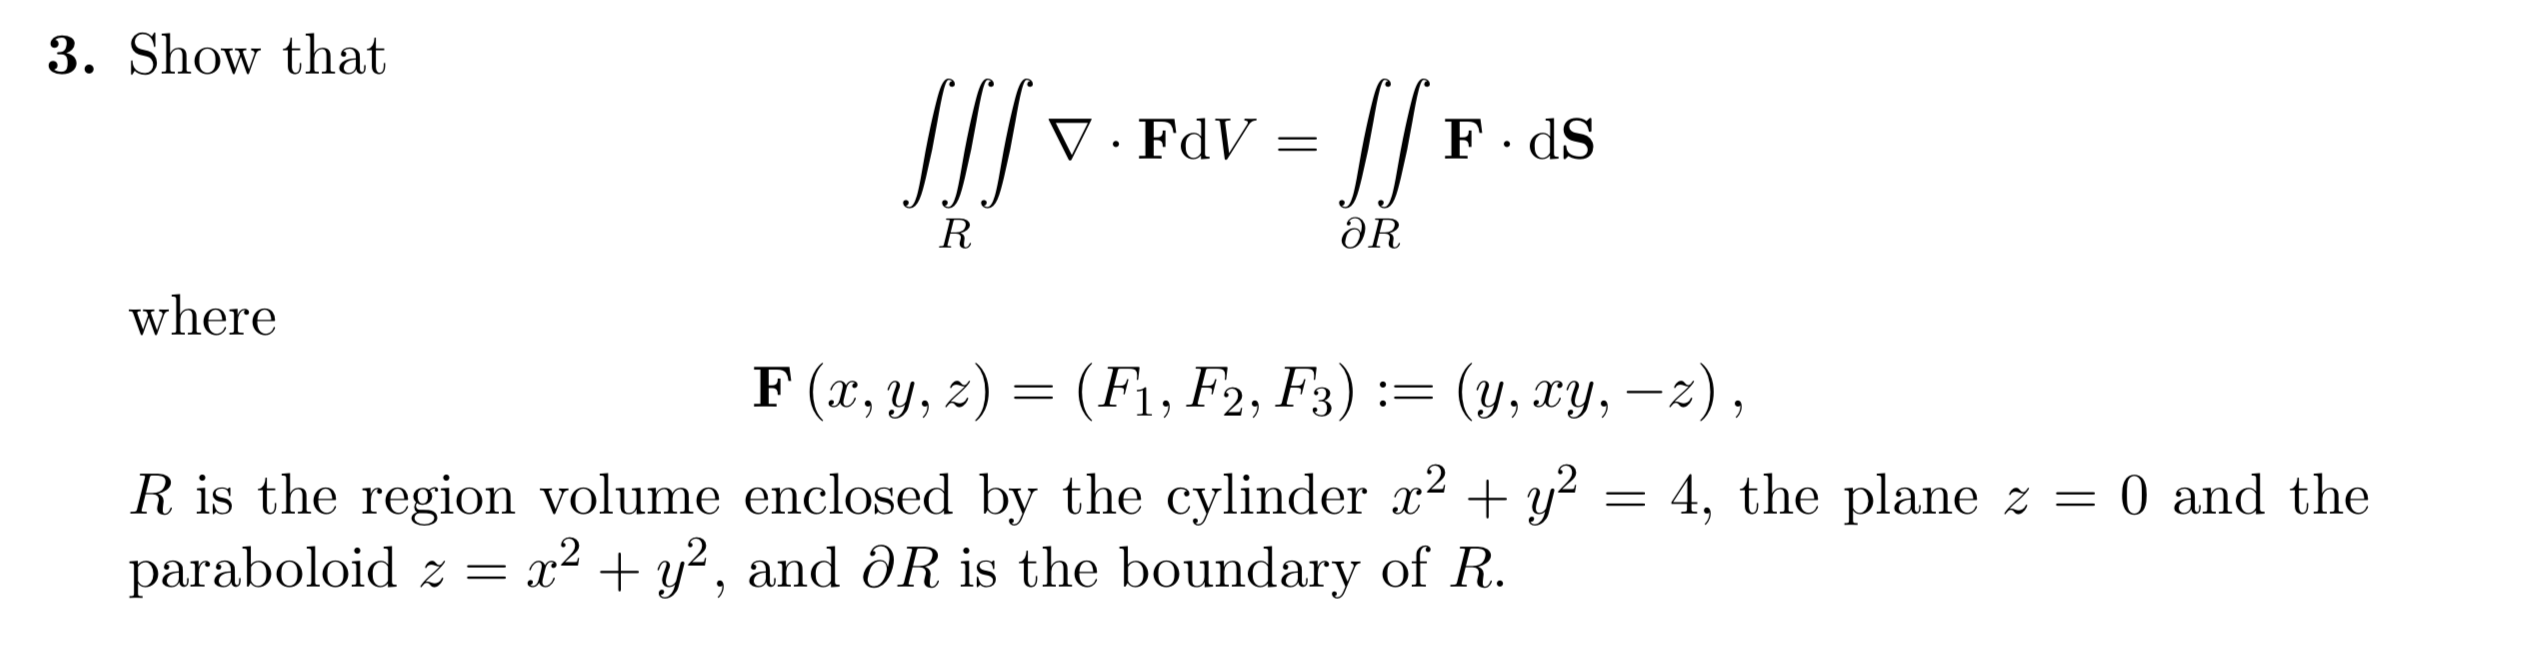
\includegraphics[width=400pt]{img/oxford-prelims-M5-multivariable-calc-6-3.png}
\end{mdframed}

\subsection{}
\begin{mdframed}
  
\includegraphics[width=400pt]{img/oxford-prelims-M5-multivariable-calc-6-4.png}
\end{mdframed}

\subsection{}
\begin{mdframed}
  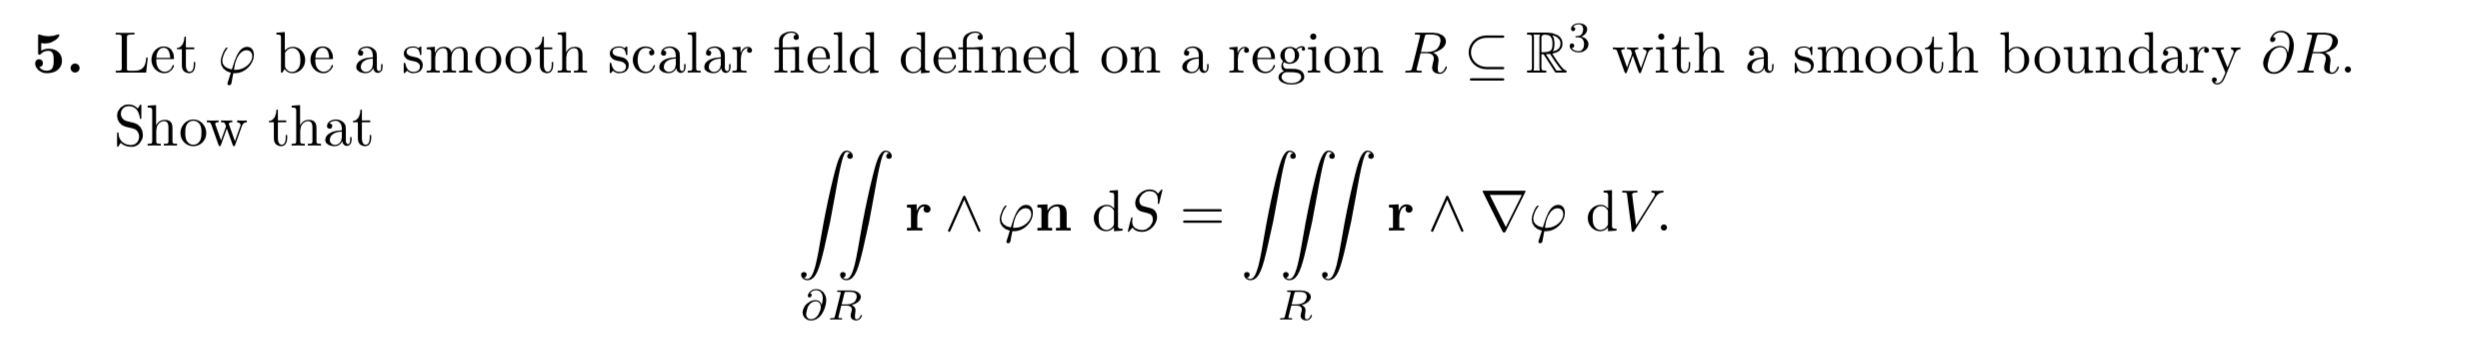
\includegraphics[width=400pt]{img/oxford-prelims-M5-multivariable-calc-6-5.png}
\end{mdframed}

\newpage
\section{Sheet 7}

\subsection{}
\begin{mdframed}
  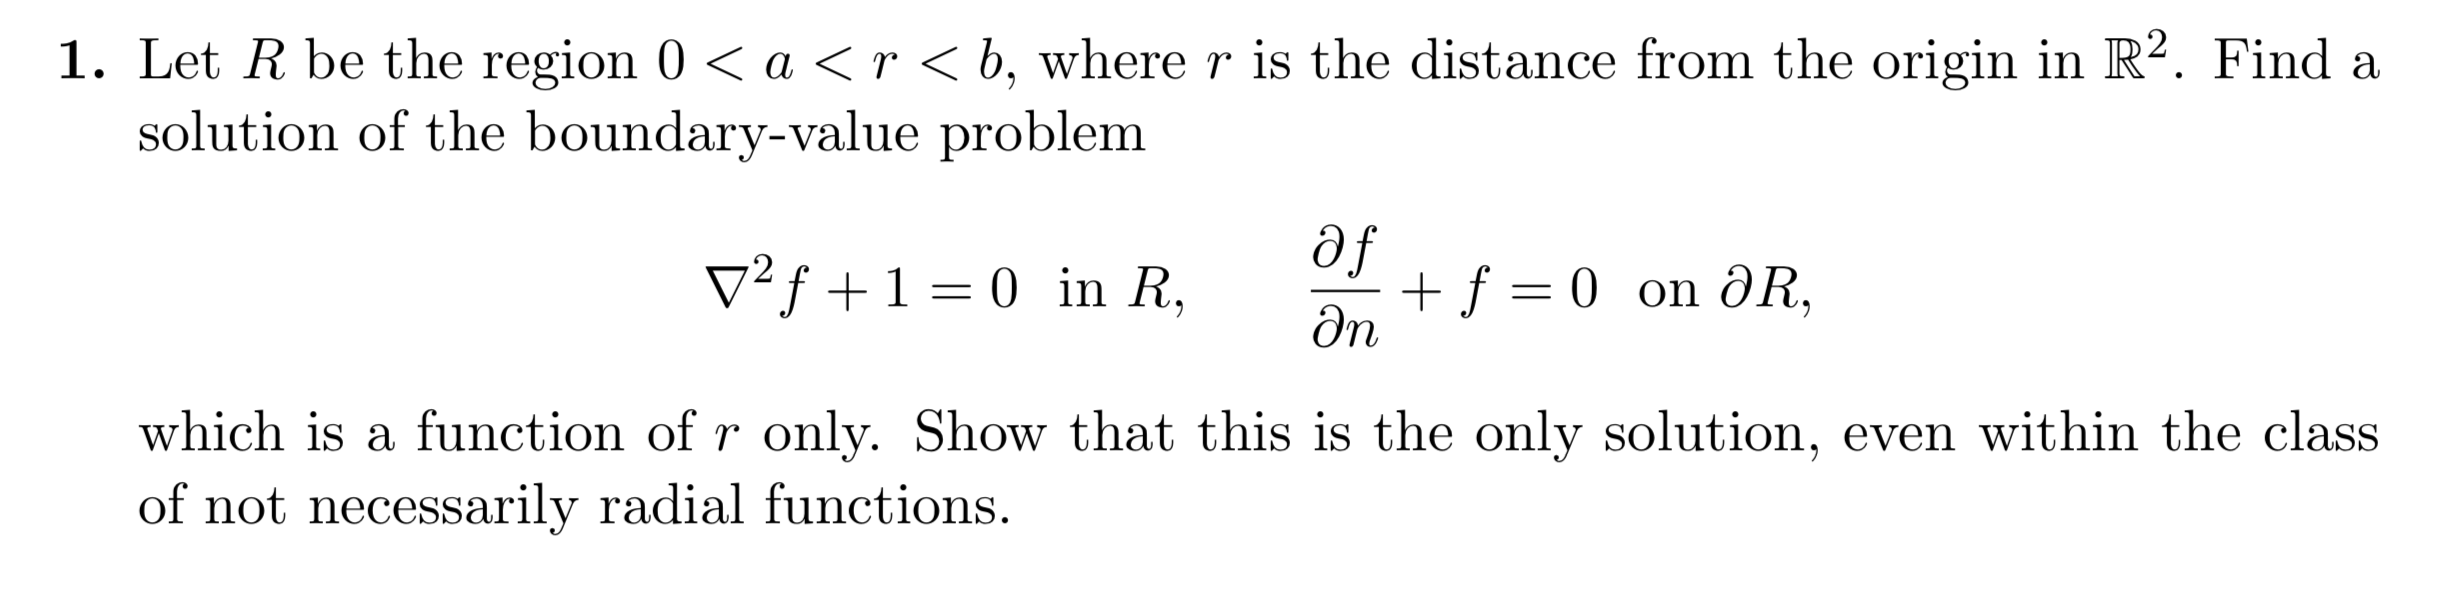
\includegraphics[width=400pt]{img/oxford-prelims-M5-multivariable-calc-7-1.png}
\end{mdframed}

\subsection{}
\begin{mdframed}
  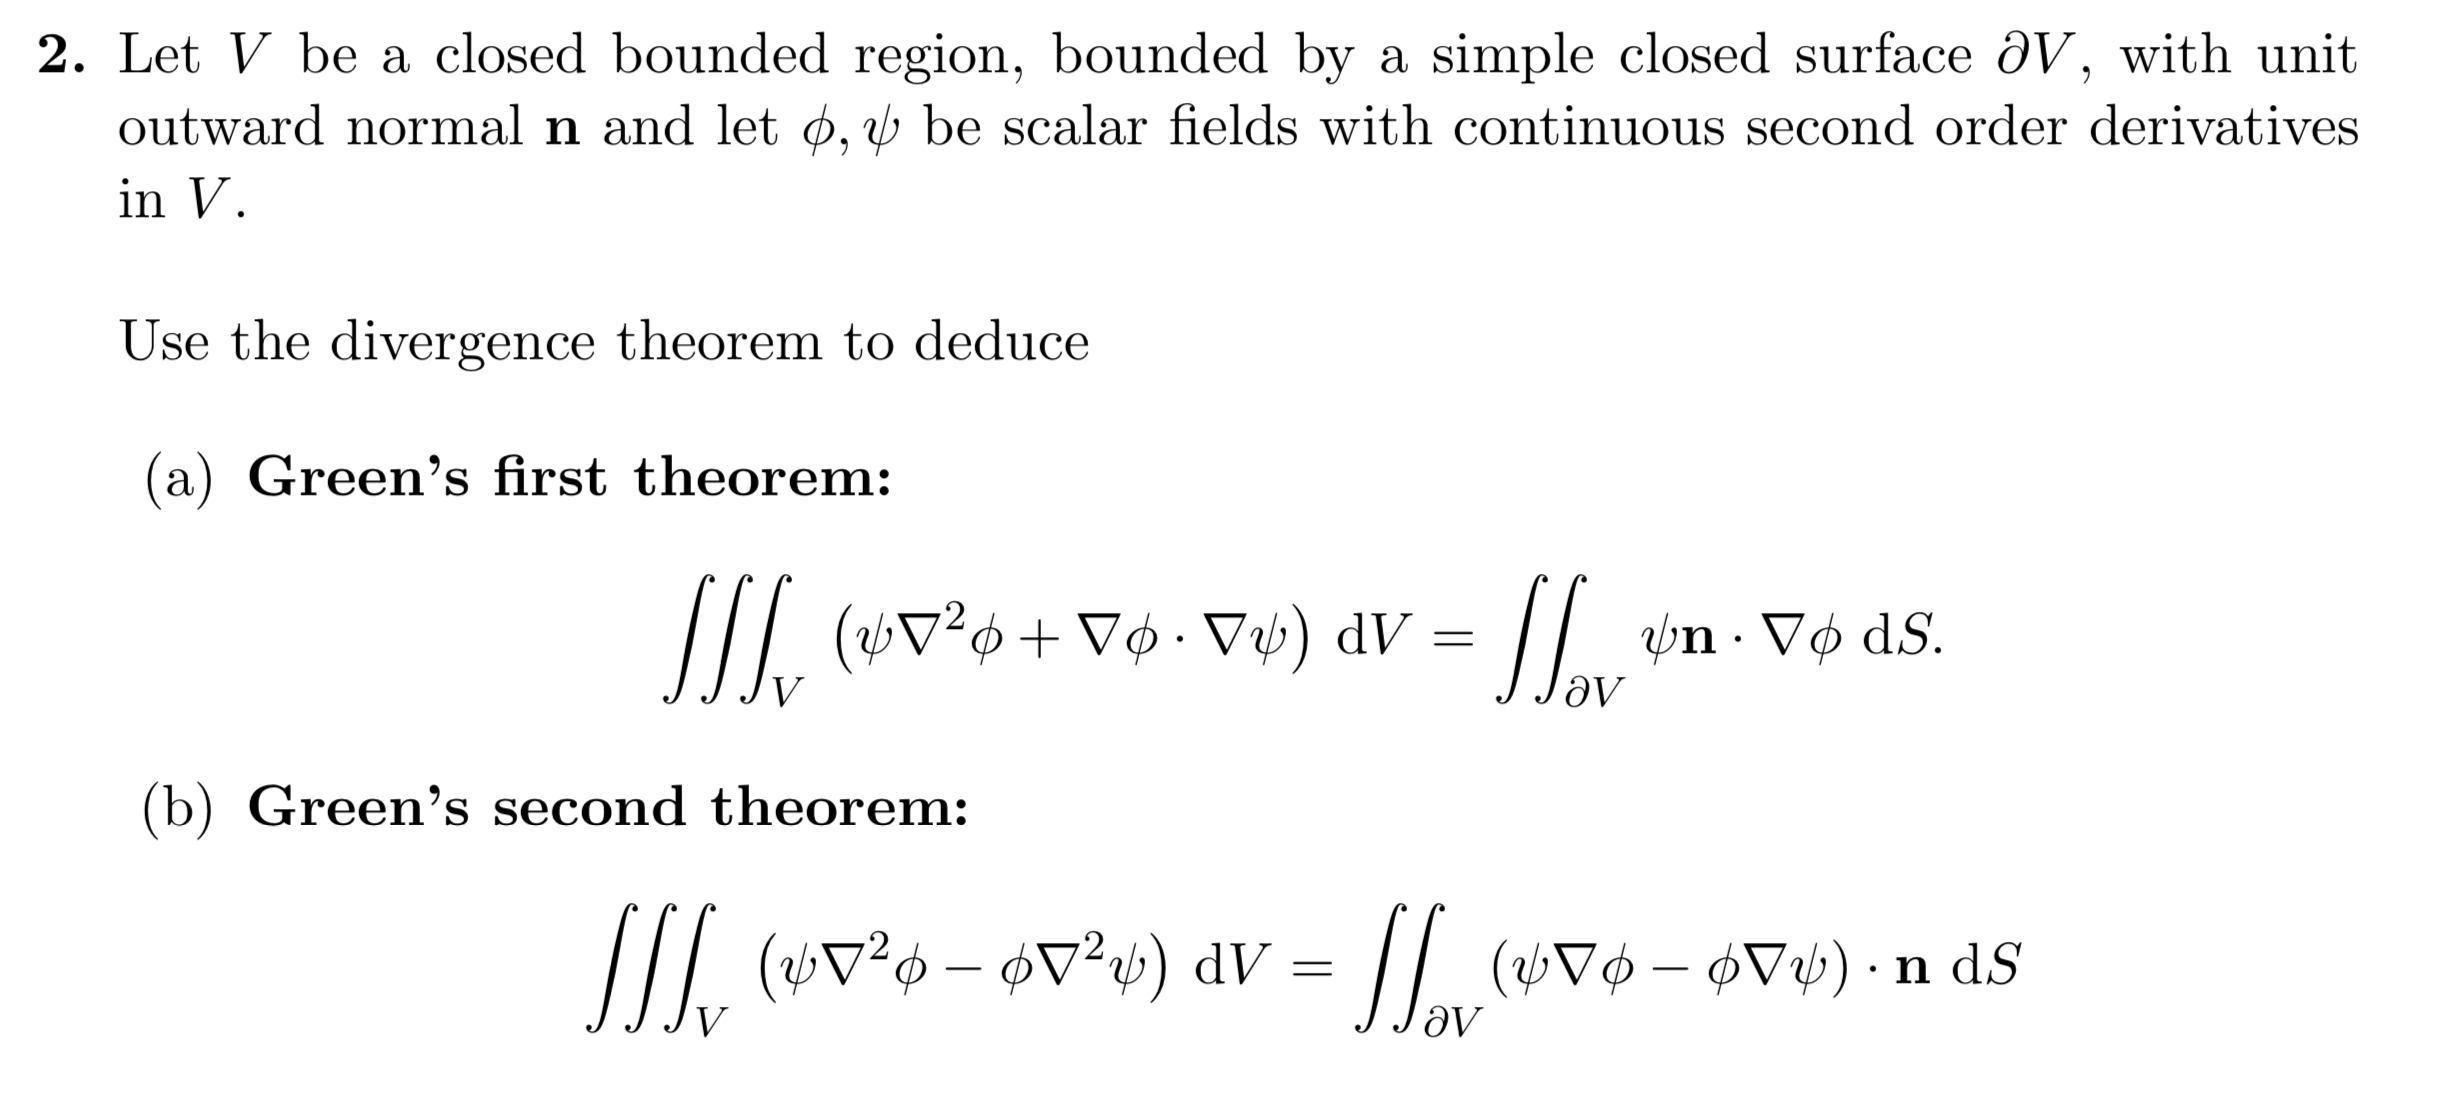
\includegraphics[width=400pt]{img/oxford-prelims-M5-multivariable-calc-7-2.png}
\end{mdframed}

\subsection{}
\begin{mdframed}
  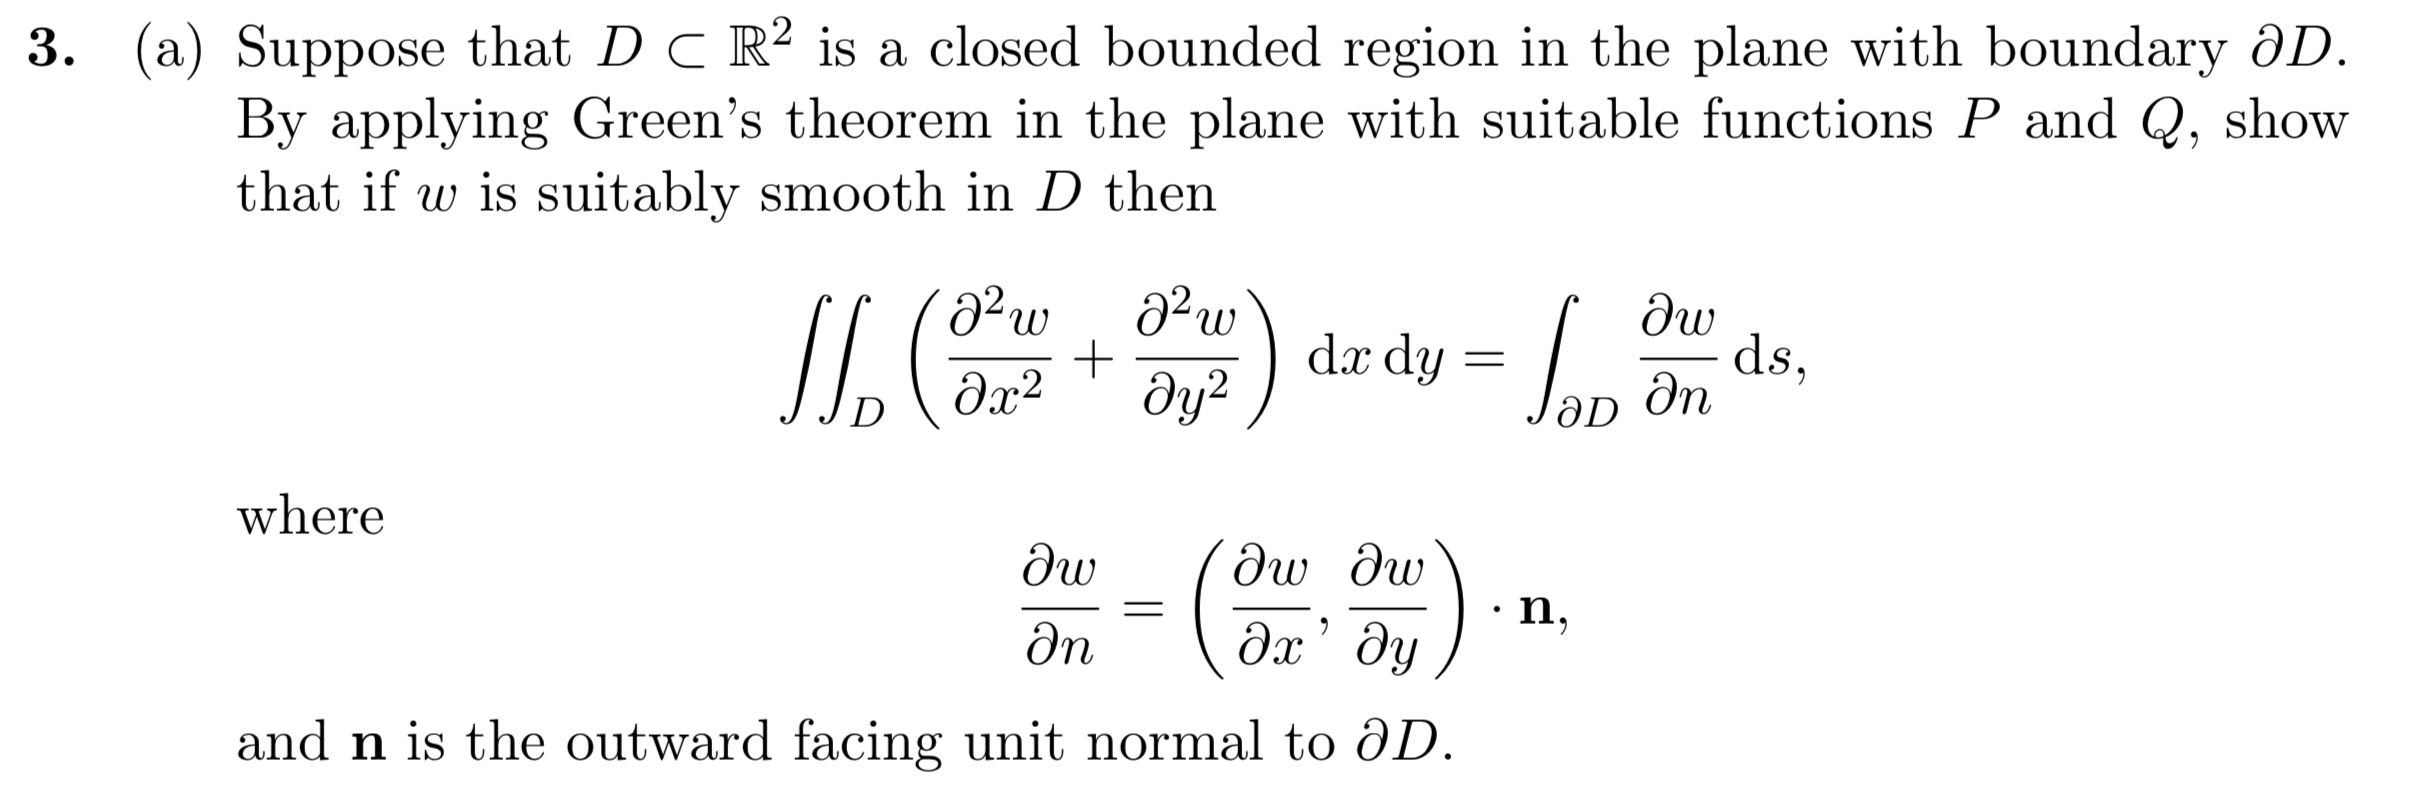
\includegraphics[width=400pt]{img/oxford-prelims-M5-multivariable-calc-7-3-a.png}
\end{mdframed}

\begin{mdframed}
  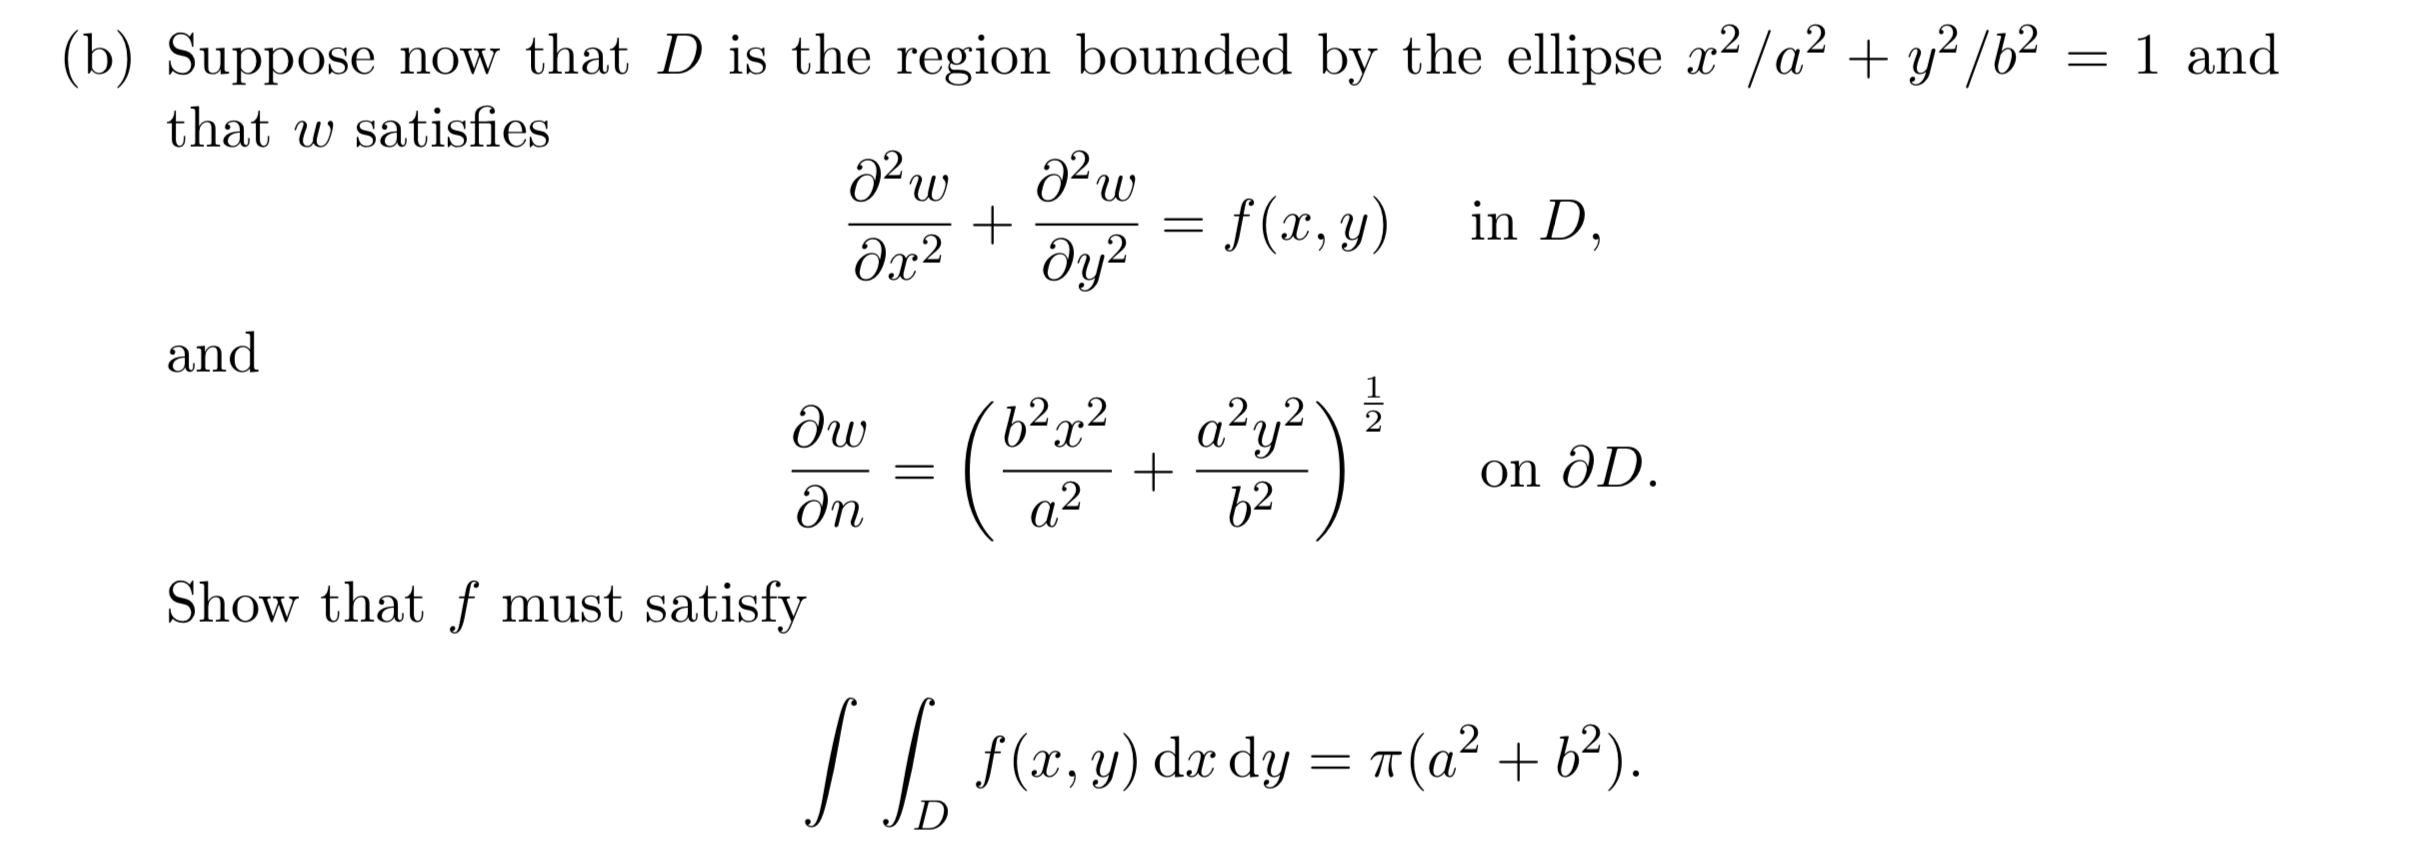
\includegraphics[width=400pt]{img/oxford-prelims-M5-multivariable-calc-7-3-b.png}
\end{mdframed}

\subsection{}
\begin{mdframed}
  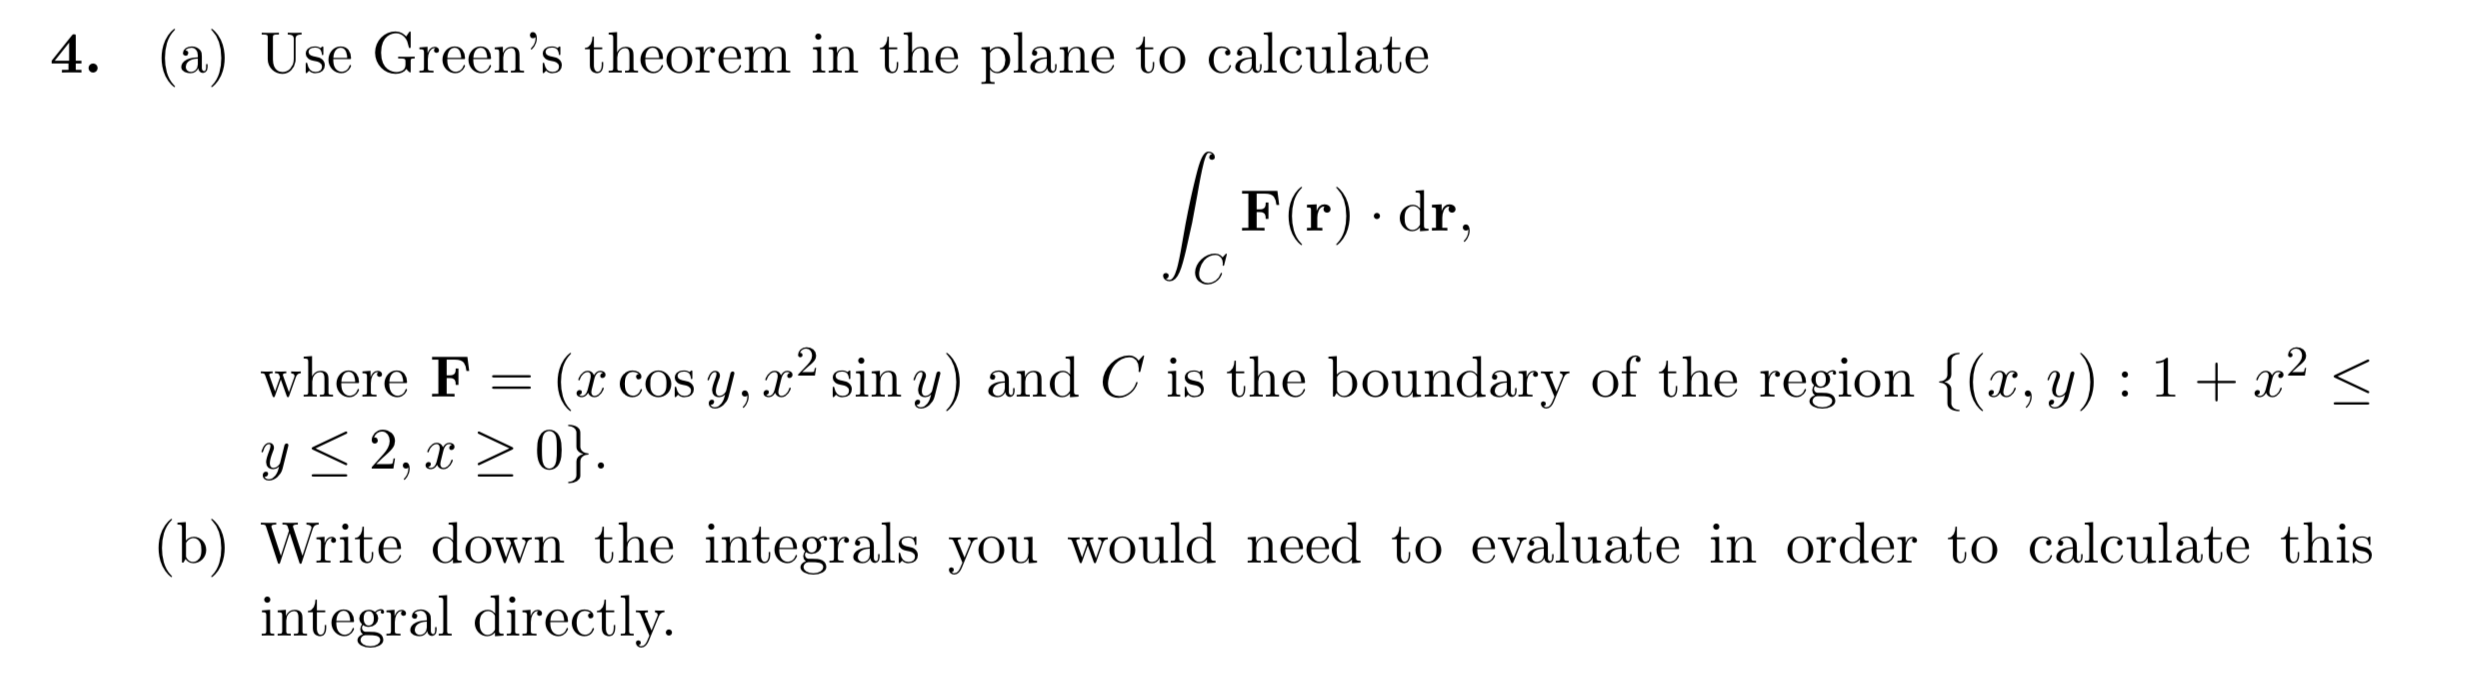
\includegraphics[width=400pt]{img/oxford-prelims-M5-multivariable-calc-7-4.png}
\end{mdframed}

\subsection{}
\begin{mdframed}
  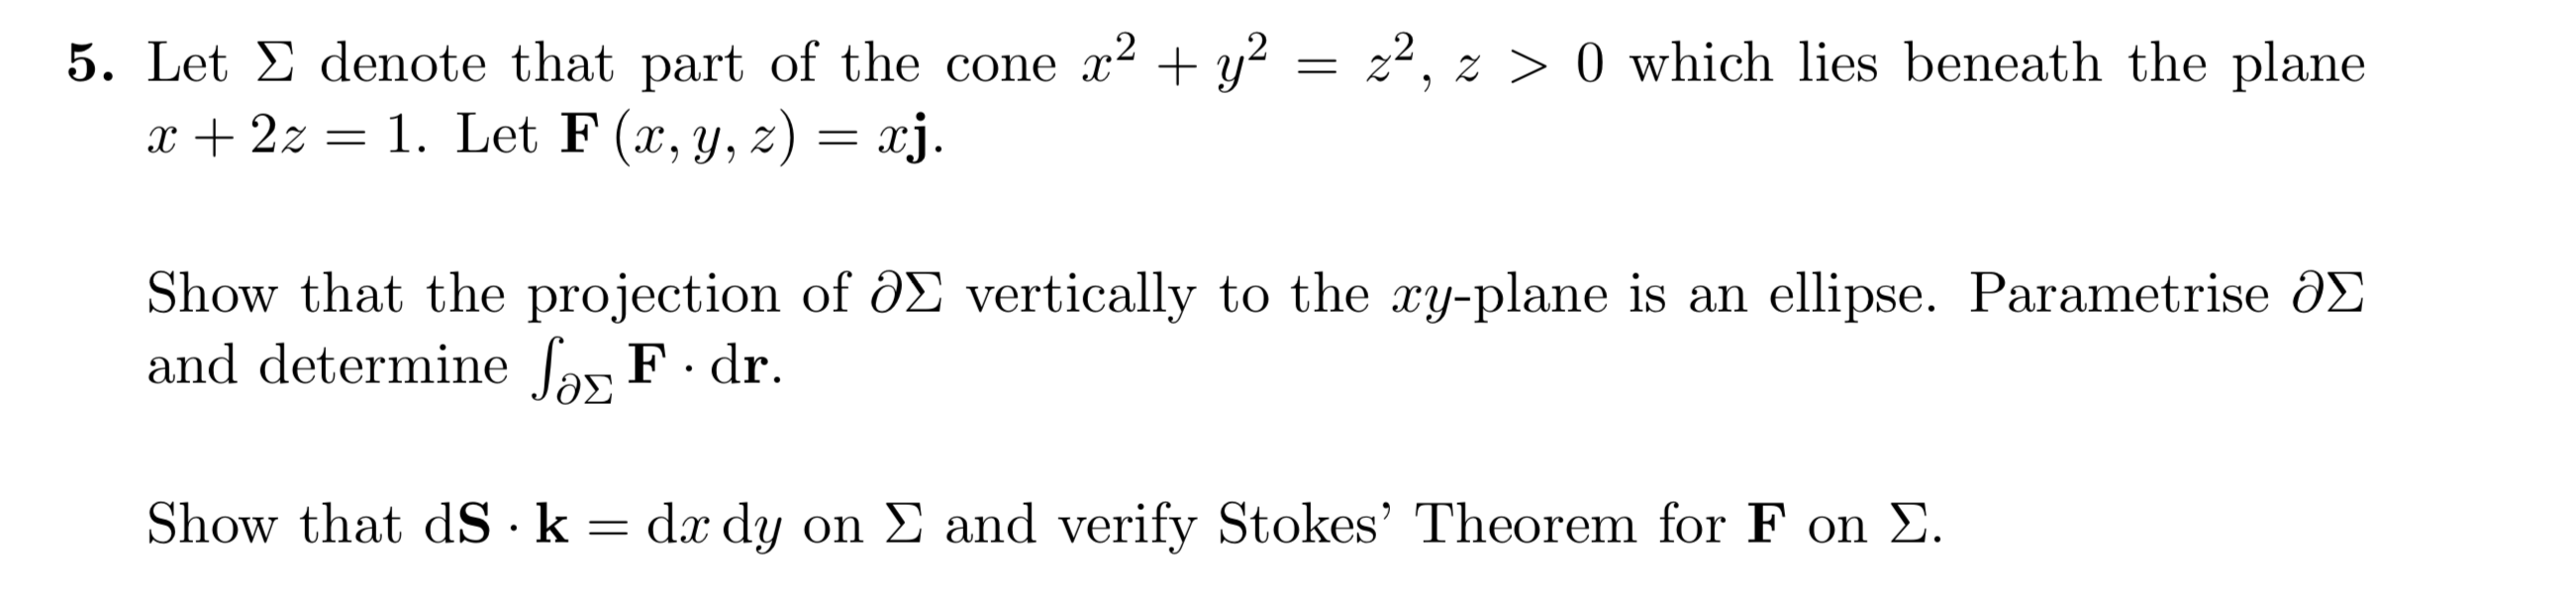
\includegraphics[width=400pt]{img/oxford-prelims-M5-multivariable-calc-7-5.png}
\end{mdframed}


\newpage
\section{Sheet 8}

\subsection{}
\begin{mdframed}
  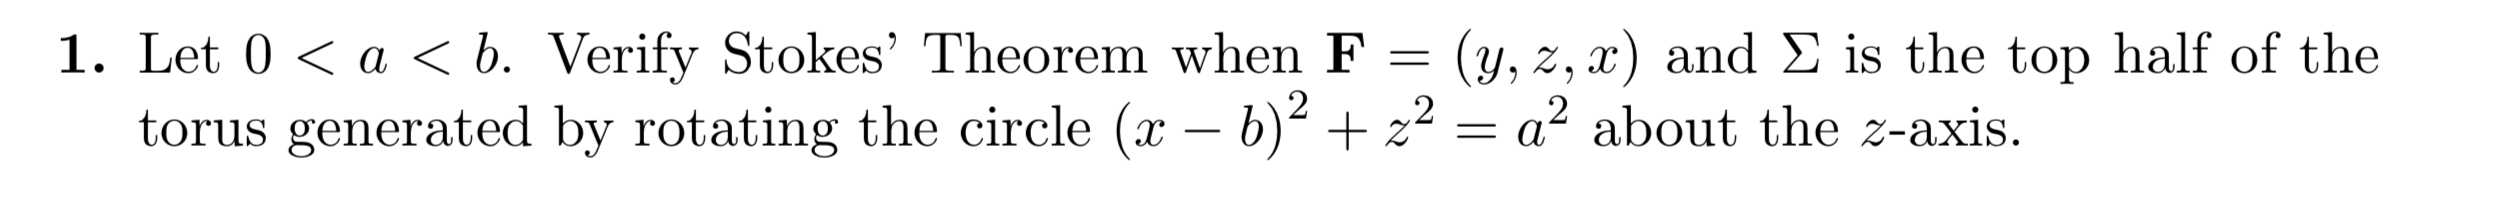
\includegraphics[width=400pt]{img/oxford-prelims-M5-multivariable-calc-8-1.png}
\end{mdframed}

\subsection{}
\begin{mdframed}
  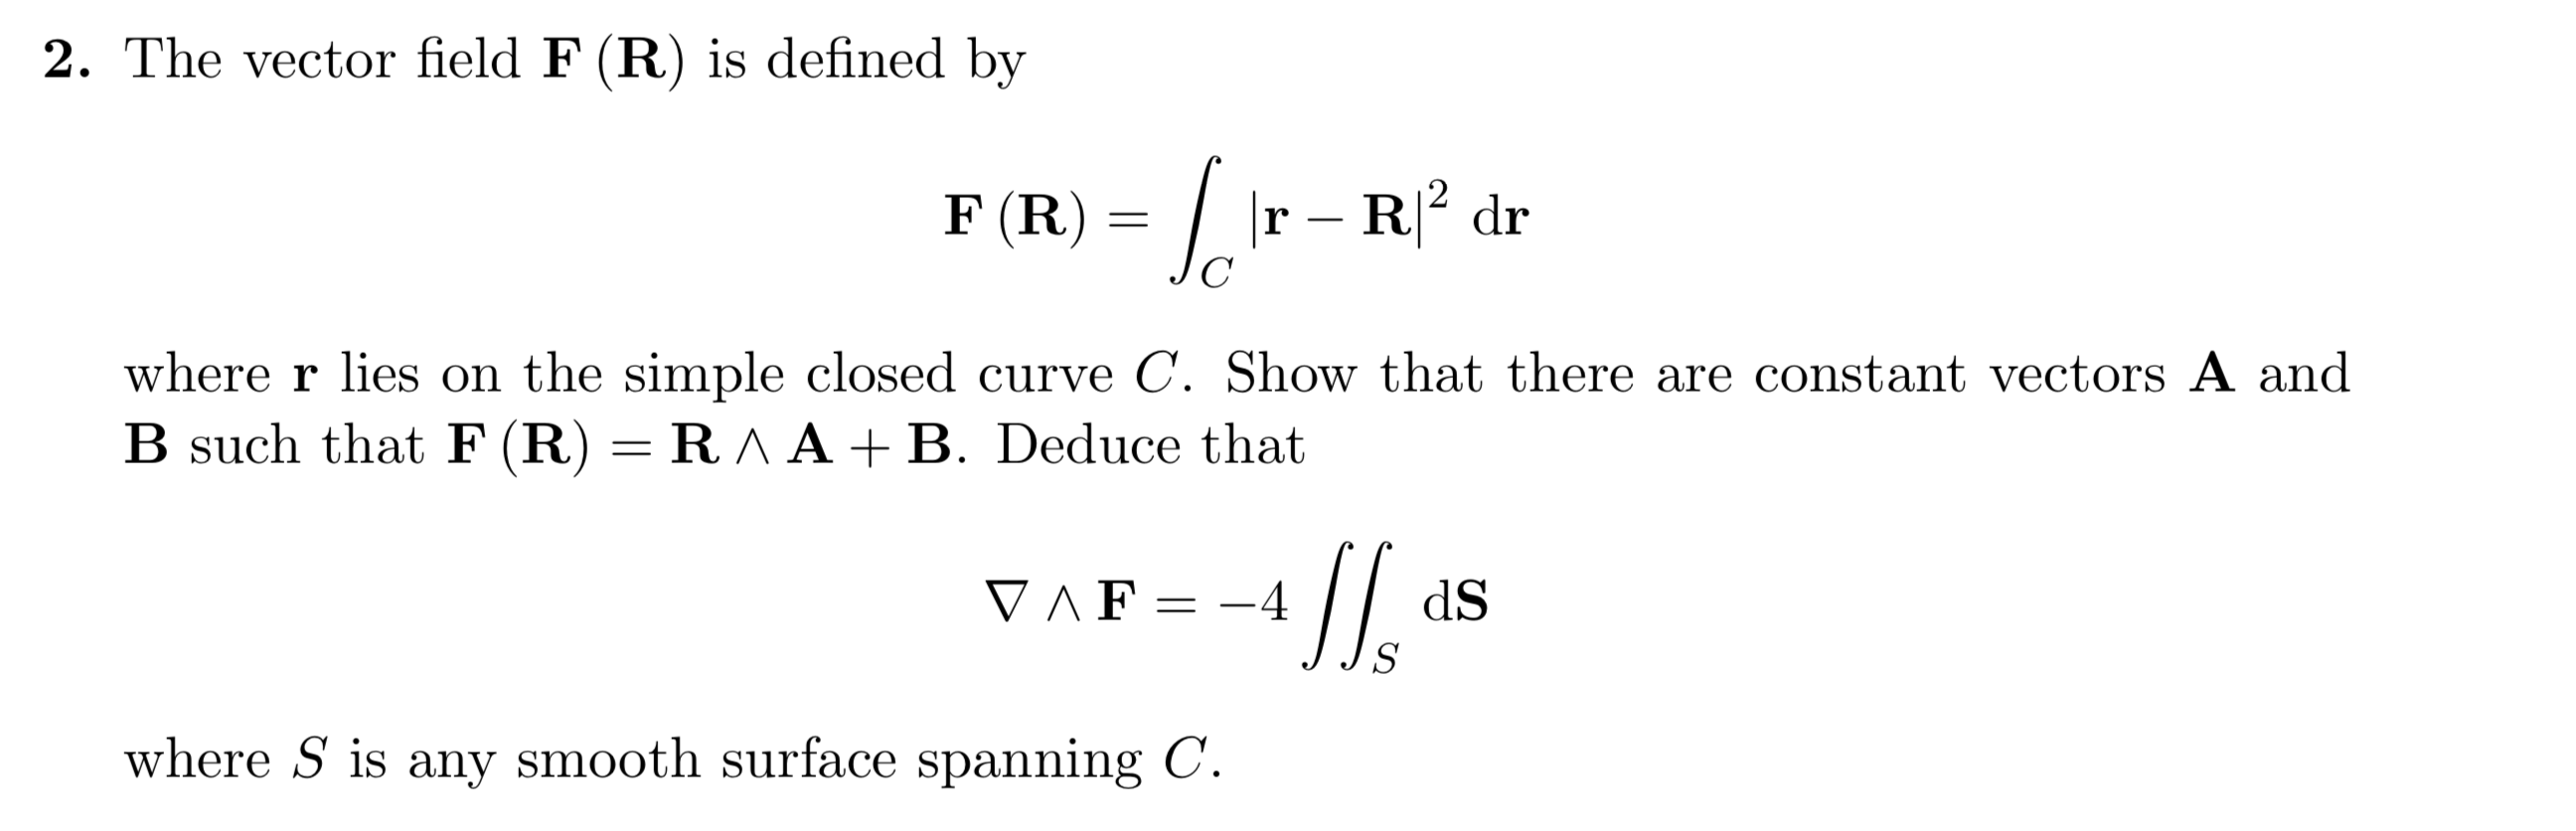
\includegraphics[width=400pt]{img/oxford-prelims-M5-multivariable-calc-8-2.png}
\end{mdframed}

\subsection{}
\begin{mdframed}
  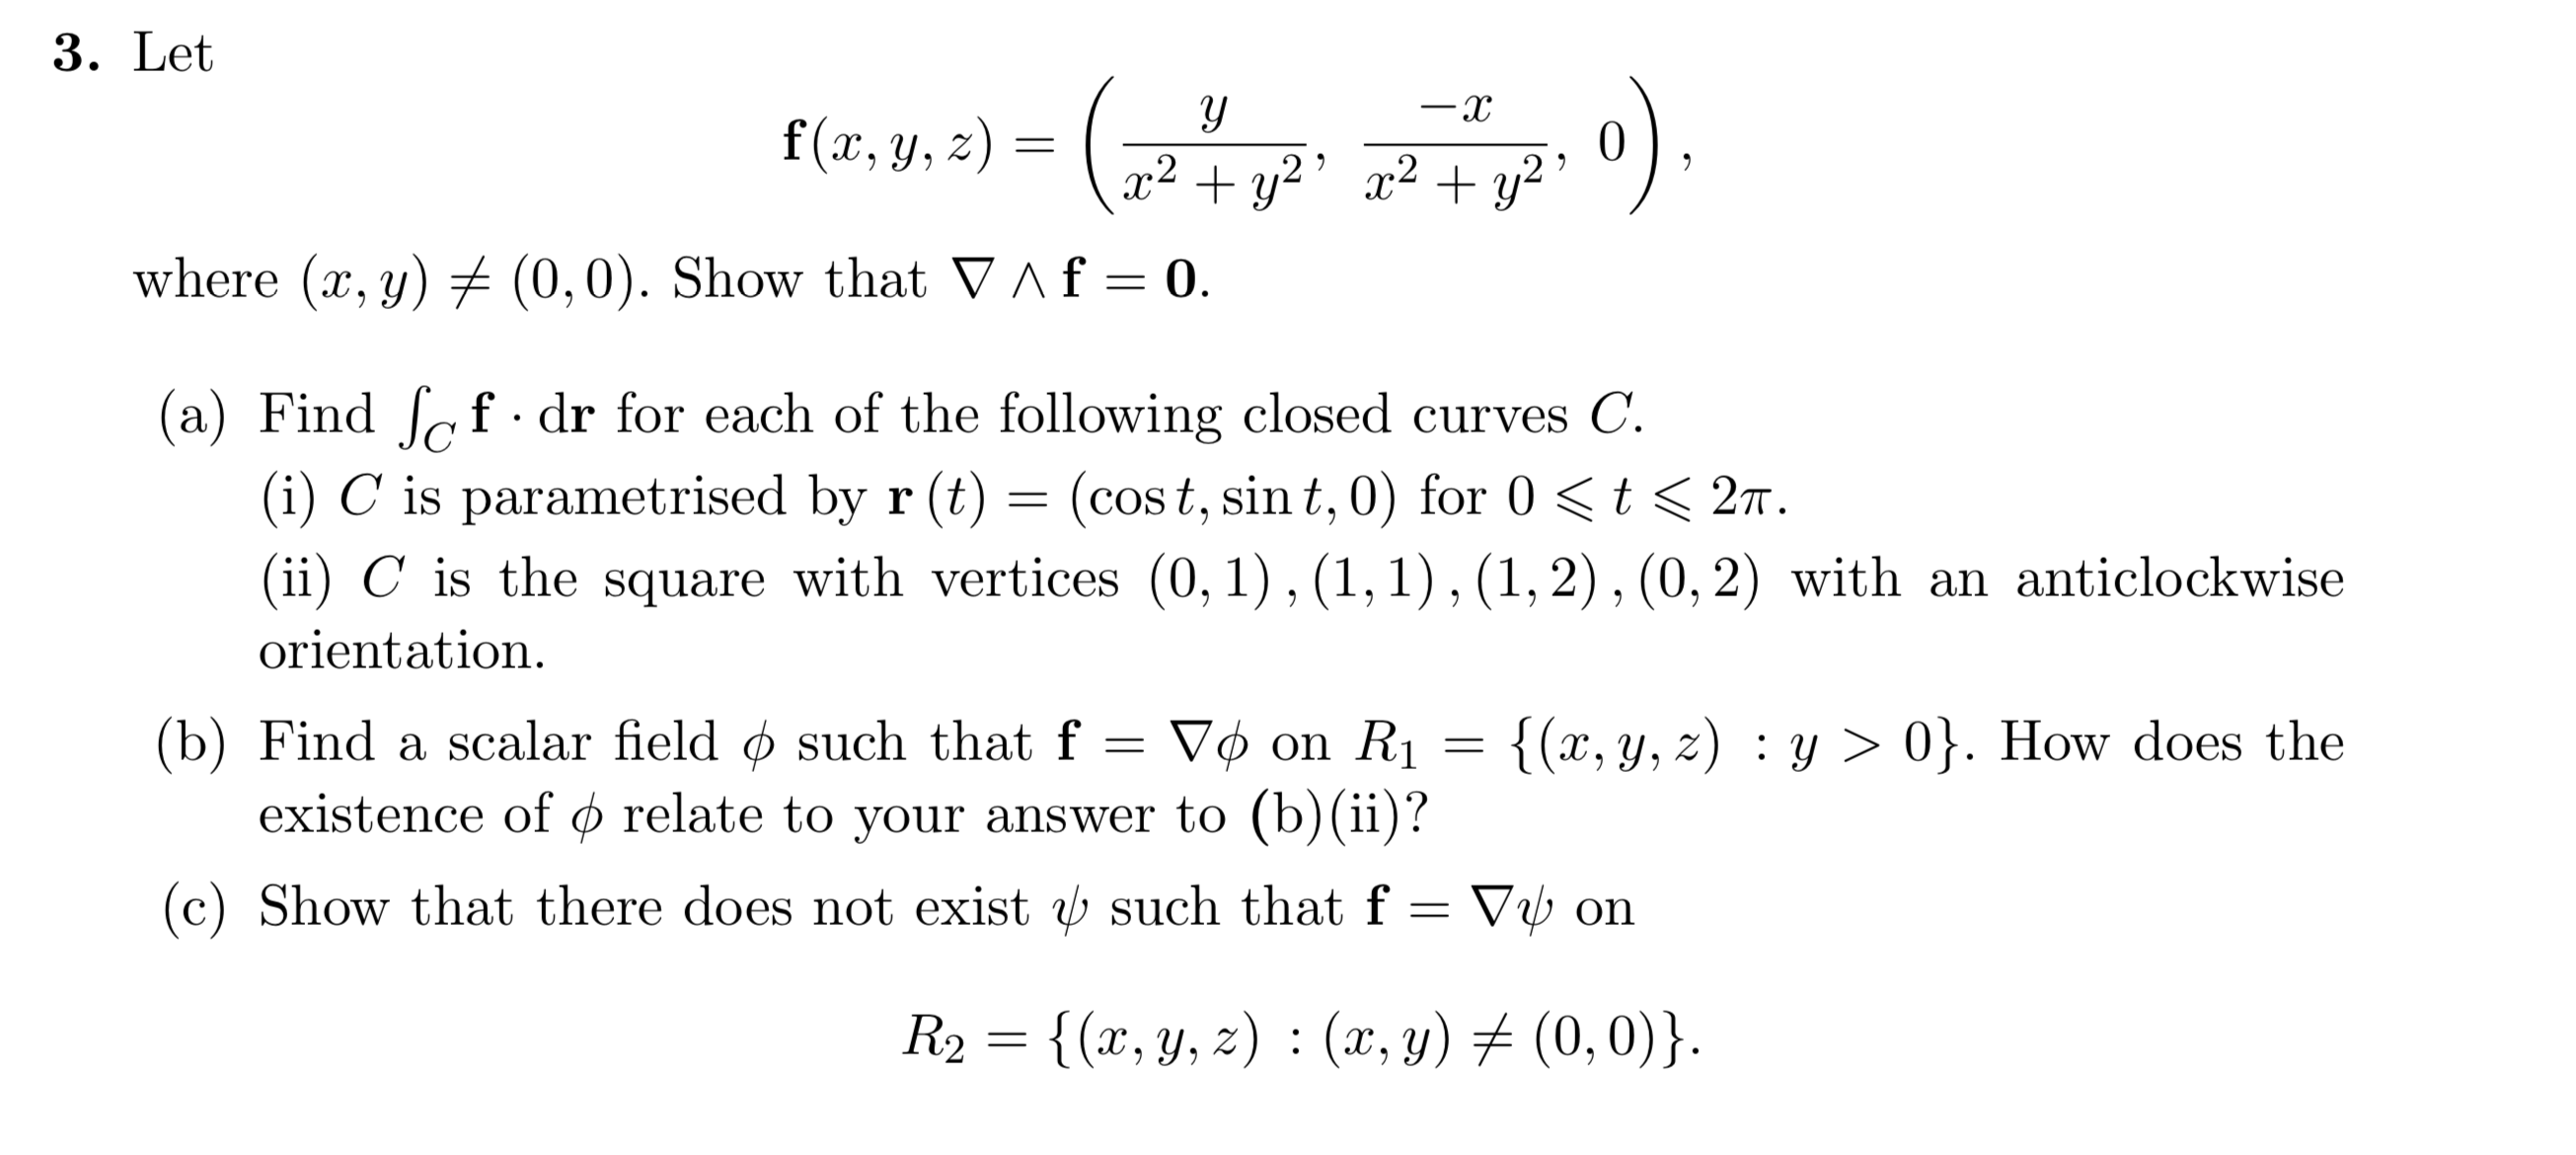
\includegraphics[width=400pt]{img/oxford-prelims-M5-multivariable-calc-8-3.png}
\end{mdframed}

\subsection{}
\begin{mdframed}
  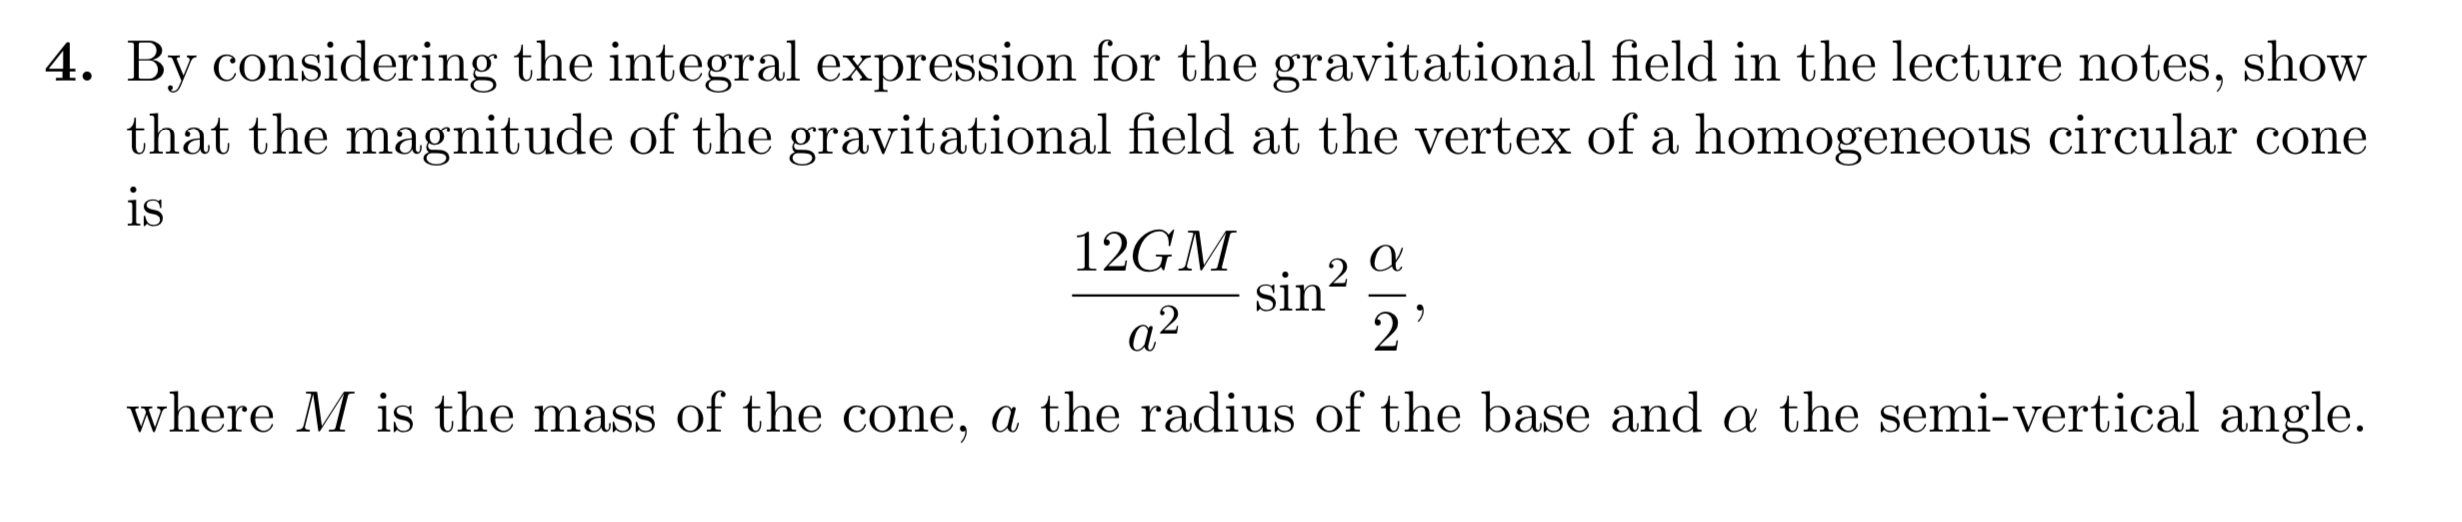
\includegraphics[width=400pt]{img/oxford-prelims-M5-multivariable-calc-8-4.png}
\end{mdframed}

\subsection{}
\begin{mdframed}
  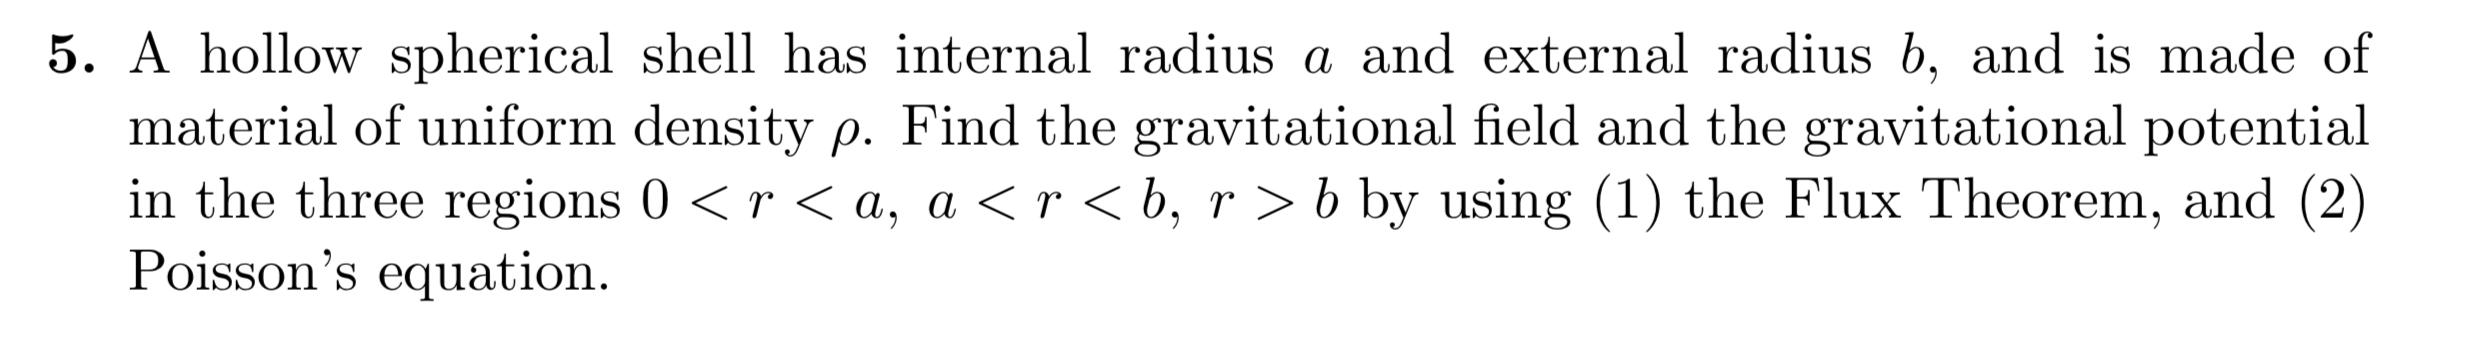
\includegraphics[width=400pt]{img/oxford-prelims-M5-multivariable-calc-8-5.png}
\end{mdframed}
